\documentclass{gtpart}
\usepackage{amsmath,amssymb,amsthm,stmaryrd}
\usepackage[all]{xy}
\usepackage[usenames,dvipsnames]{xcolor}
\usepackage{tikz}
\usetikzlibrary{shapes,positioning,fit}
\usepackage{url}
\usepackage{hyperref}
\usepackage{enumerate}
\usepackage{tensor}
%/home/grad/zyf/TeX/inputs/
\usepackage{mathrsfs}
\usepackage{graphicx}
\usepackage{mathtools}
\usetikzlibrary{arrows}
%\usepackage{amsrefs}
%\usepackage{setspace}
%\doublespacing

\title{The Hecke algebra action on Morava $E$-theory of height $2$}
\author{Yifei Zhu}
% \givenname{Yifei}
% \surname{Zhu}
% \address{Department of Mathematics\\Northwestern University\\\newline 
% 2033 Sheridan Road\\Evanston\\IL 60208\\USA}
% \email{zyf@math.northwestern.edu}
% \urladdr{http://www.math.northwestern.edu/~zyf}

%\subject{primary}{msc2000}{55P99}
%\subject{secondary}{msc2000}{55Q99}

%\bibliographystyle{gtart}
\parskip 0.7pc
\parindent 0pt

\newtheorem{thm}{Theorem}
\newtheorem{cor}[thm]{Corollary}
\newtheorem{prop}[thm]{Proposition}
\newtheorem{lem}[thm]{Lemma}
\theoremstyle{definition}
\newtheorem{defn}[thm]{Definition}
\newtheorem{cstr}[thm]{Construction}
\theoremstyle{remark}
\newtheorem{rmk}[thm]{Remark}
\newtheorem{ex}[thm]{Example}
\newtheorem{case}[thm]{Case}
\newtheorem{slogan}[thm]{Slogan}
\newtheorem{ques}[thm]{Question}

\def\co{\colon\thinspace}
\newcommand{\mb}[1]{\mathbb{#1}}
\newcommand{\mf}[1]{\mathfrak{#1}}
\newcommand{\Hom}{\ensuremath{{\rm Hom}}}
\newcommand{\Aut}{{\rm Aut}}
\newcommand{\Gal}{{\rm Gal}}
\newcommand{\LT}{{\rm LT}}
\newcommand{\Spec}{{\rm Spec\thinspace}}
\newcommand{\Proj}{{\rm Proj\thinspace}}
\newcommand{\Spf}{{\rm Spf\thinspace}}
\newcommand{\Ell}{{\rm Ell}}
\newcommand{\Sch}{{\rm Sch}}
\newcommand{\cF}{\overline {\mb F}}
\newcommand{\ck}{\overline k}
\newcommand{\CA}{{\cal A}}
\newcommand{\CB}{{\cal B}}
\newcommand{\CC}{{\cal C}}
\newcommand{\CE}{{\cal E}}
\newcommand{\CF}{{\cal F}}
\newcommand{\CG}{{\cal G}}
\newcommand{\CH}{{\cal H}}
\newcommand{\CHom}{{\cal H}om}
\newcommand{\CLie}{{\cal L}ie}
\newcommand{\CM}{{\cal M}}
\newcommand{\CMB}{\overline {\cal M}}
\newcommand{\CO}{{\cal O}}
\newcommand{\CP}{{\cal P}}
\newcommand{\CS}{{\cal S}}
\newcommand{\FF}{{\mf F}}
\newcommand{\Mod}{{\rm Mod}}
\newcommand{\Alg}{{\rm Alg}}
\newcommand{\dl}{{\rm DL}}
\newcommand{\Set}{{\rm Set}}
\newcommand{\Sq}{{\rm Sq}}
\newcommand{\Frob}{{\rm Frob}}
\newcommand{\DF}{{{\rm DefFrob}_\BG}}
\newcommand{\Model}{{\rm Model}}
\newcommand{\HGa}{{\widehat{\mb G}_a}}
\newcommand{\HGm}{{\widehat{\mb G}_m}}
\newcommand{\Gm}{{{\mb G}_m}}
\newcommand{\DL}{Dyer-Lashof~}
\newcommand{\EM}{Eilenberg-Mac~Lane~}
\newcommand{\BC}{{\mb C}}
\newcommand{\BE}{{\mb E}}
\newcommand{\BF}{{\mb F}}
\newcommand{\BG}{{\mb G}}
\newcommand{\BN}{{\mb N}}
\newcommand{\BP}{{\mb P}}
\newcommand{\BQ}{{\mb Q}}
\newcommand{\BR}{{\mb R}}
\newcommand{\BS}{{\mb S}}
\newcommand{\BW}{{\mb W}}
\newcommand{\BZ}{{\mb Z}}
\newcommand{\fm}{{\mf m}}
\newcommand{\HC}{\widehat{C~}\!}
\newcommand{\HCC}{\widehat{~\!\!\CC}}
\newcommand{\HE}{\widehat{E~}\!}
\newcommand{\Hf}{\widehat{f}}
\newcommand{\Hphi}{\widehat{\phi}}
\newcommand{\Hpsi}{\widehat{\psi}}
\newcommand{\HS}{\widehat{S~}\!}
\newcommand{\TA}{\tilde{\A}}
\newcommand{\Tc}{\tilde{c}}
\newcommand{\TE}{\widetilde{E\thinspace}\!}
\newcommand{\Tf}{\widetilde{f}}
\newcommand{\Tp}{\widetilde{\psi}}
\newcommand{\TW}{\widetilde{W\thinspace}\!}
\newcommand{\md}{~~{\rm mod}~}
\newcommand{\ad}{{\rm and}}
\newcommand{\can}{{\rm can}}
\newcommand{\HT}{{\rm ht}}
\newcommand{\id}{{\rm id}}
\newcommand{\op}{{\rm op}}
\newcommand{\tf}{{\rm tf}}
\newcommand{\TMF}{{\rm TMF}}
\newcommand{\tmf}{{\rm tmf}}
\newcommand{\MF}{{\rm MF}}
\newcommand{\tr}{{\rm trace}}
\newcommand{\univ}{{\rm univ}}
\newcommand{\Ext}{{\rm Ext}}
\newcommand{\Tor}{{\rm Tor}}
\newcommand{\nul}{{\rm nul}}
\newcommand{\A}{\alpha}
\newcommand{\B}{\beta}
\renewcommand{\D}{\Delta}
\renewcommand{\d}{\delta}
\newcommand{\f}{\phi}
\newcommand{\G}{\Gamma}
\newcommand{\g}{\gamma}
\newcommand{\K}{\kappa}
\renewcommand{\l}{\lambda}
\renewcommand{\o}{\omega}
\newcommand{\ou}{\underline{\omega\!}}
\newcommand{\si}{\sigma}
\newcommand{\T}{\tau}
\newcommand{\om}{\underline{\omega\!}_{~E/S}}
\newcommand{\p}{\psi^3}
\newcommand{\s}{S^\bullet}
\newcommand{\ce}{\coloneqq}
\newcommand{\lb}{\llbracket}
\newcommand{\rb}{\rrbracket}
\newcommand{\lp}{(\!(}
\newcommand{\rp}{)\!)}
\newcommand{\Ht}{\widehat{T}}
\newcommand{\Tt}{\widetilde{T}}
\newcommand{\mt}{\widetilde{m}}
\newcommand{\lt}{\widetilde{\lambda}}
\newcommand{\todo}{\spadesuit}
\newcommand{\totodo}{\heartsuit}
\renewcommand{\=}{\approx}
\renewcommand{\-}{\sim}
\newcommand{\isog}[1]{Proposition \ref{prop:isog}\thinspace \eqref{isog(#1)}}
\newcommand{\q}[1]{Proposition \ref{prop:Q}\thinspace \eqref{Q(#1)}}
\newcommand{\go}[1]{Definition \ref{def:go}\thinspace \eqref{go(#1)}}
\newcommand{\rd}[1]{\textcolor{red}{#1}}
\newcommand{\bl}[1]{\textcolor{blue}{#1}}
\newcommand{\wt}[1]{\textcolor{white}{#1} \!~}
\newcommand{\gl}{{\rm gl}}
\newcommand{\GL}{{\rm GL}}
\newcommand{\SL}{{\rm SL}}
\newcommand{\Tate}{{\rm Tate}}

\makeatletter
\DeclareRobustCommand\widecheck[1]{{\mathpalette\@widecheck{#1}}}
\def\@widecheck#1#2{%
    \setbox\z@\hbox{\m@th$#1#2$}%
    \setbox\tw@\hbox{\m@th$#1%
       \widehat{%
          \vrule\@width\z@\@height\ht\z@
          \vrule\@height\z@\@width\wd\z@}$}%
    \dp\tw@-\ht\z@
    \@tempdima\ht\z@ \advance\@tempdima2\ht\tw@ \divide\@tempdima\thr@@
    \setbox\tw@\hbox{%
       \raise\@tempdima\hbox{\scalebox{1}[-1]{\lower\@tempdima\box
\tw@}}}%
    {\ooalign{\box\tw@ \cr \box\z@}}}
\makeatother

\numberwithin{equation}{section}
\renewcommand{\theequation}{\thesection.\arabic{equation}}
\numberwithin{thm}{section}


\begin{document}



\begin{abstract}
 \centerline{\textbf{\today}}\vspace{.5in}

 Given a one-dimensional formal group of height 2, 
 let $E$ be the Morava $E$-theory spectrum associated to its universal deformation over the Lubin-Tate ring.  
 By computing with moduli spaces of elliptic curves, 
 we give an explicitation for an algebra of Hecke operators acting on $E$-cohomology.  
 This leads to a vanishing result for Rezk's logarithmic cohomology operation on the units of $E$.  
 It identifies a family of elements in the kernel with meromorphic modular forms whose Serre derivative is zero.  
 Our calculation finds a connection to logarithms of modular units.  
 In particular, we work out an action of Hecke operators on Knopp and Mason's logarithmic $q$-series 
 that agrees with our vanishing result and extends the classical Hecke action on modular forms.  
\end{abstract}

\maketitle



\section{Introduction}

In the context of elliptic cohomology, Hecke operators have been studied as cohomology 
operations by Baker \cite{Baker90,Baker89}, Ando \cite{Ando95}, and 
Ganter \cite{stringy}, among others.  The various cohomology theories each have 
as coefficients a ring of modular forms 
of a particular type---modular forms on $\SL_2(\BZ)$ with no condition at the cusp, 
$p$-adic modular forms, modular forms with level structure---or it is a 
closely related ring, e.g., a completion of the former at an ideal.  These cohomology 
theories are topological realizations of the domain that Hecke operators act on.  

The notion of an elliptic spectrum \cite[Definition 1.2]{AHS01} and the theory of multiplicative ring 
spectra, notably the theorem of Goerss, Hopkins, and Miller \cite[Corollary 7.6]{GH}, enable 
studying this action of Hecke operators via power operations.  
These operations arise from the multiplicative ring structure on a spectrum, 
and they capture all the algebraic structure that naturally adheres to the cohomology theory represented by the spectrum \cite{H_infty}.  

In particular, Morava $E$-theories are a family 
of cohomology theories whose power operations 
are better understood thanks to the work of Ando, Hopkins, Strickland, and Rezk \cite{AHS04,cong,h2}.  
This family is organized by heights $n$ and primes $p$.  
Here the theory of formal groups plays a key 
role: each $E$-theory spectrum $E$ corresponds to a specific 
one-dimensional commutative formal group, whose finite 
flat subgroups, in turn, correspond precisely to power operations on $E$-cohomology.  At 
height $n = 2$, formal groups of elliptic curves provide concrete models for 
$E$-theories.  The associated power operations can then be computed from moduli spaces that 
parametrize isogenies between elliptic curves.  

In this paper, we study the action of Hecke operators on Morava $E$-theories 
at height 2, based on the explicit calculations for power operations in 
\cite{h2p2,p3}.  This is motivated by the interpretation---in terms of Hecke operators---for 
Rezk's logarithmic operations on $E$-cohomology at an arbitrary height (see 
\cite[1.12]{log}).  At height 2, these 
``logarithms'' are critical in the work of Ando, Hopkins, and Rezk on rigidification of 
the string-bordism elliptic genus, or more precisely, on $E_\infty$-string orientations 
of the spectrum of topological modular forms \cite{koandtmf}.  
For the space of such orientations, its set of components 
can be detected by elements in the kernel of a logarithm.  
Explicitly, these elements are identified with Eisenstein series $\CE_k$, which are 
eigenforms of Hecke operators [ibid., Theorem 12.3].  

In Section \ref{sec:kerlog}, we give a different account of certain elements in the kernel of a 
logarithm at height 2: they are meromorphic modular forms with vanishing Serre derivative, including 
modular forms whose zeros and poles are located only at the cusps, such as the modular discriminant $\D$.  
This is stated as Theorem \ref{thm:kerlog}.  

The discrepancy between the above two sets of elements---Eisenstein series as opposed to the 
discriminant---results from the different domains of the logarithms.  
The former is the group of units in the zeroth cohomology of an even-dimensional sphere, 
while the latter is that of the infinite-dimensional complex projective space 
$\BC\BP^\infty$; that is, the logarithms are defined on $E^0(S^{2 k})^\times$ and $E^0(\BC\BP^\infty)^\times$ respectively.  

The finiteness of $E^0(S^{2 k})$ as a module over $E^0$ puts the formula for the logarithm in a simple form.  
Specifically, the logarithm can be written as a combination of Hecke operators acting on $\log (1 + f)$, 
where $f$ is a generator of the truncated polynomial ring $E^0(S^{2 k})$.  Note that the formal power series 
expansion of $\log (1 + f)$ simply equals $f$, because $f^2 = 0$ (see \cite[Proposition 4.8 and Example 4.9]{koandtmf}).  

In the latter case of $E^0(\BC\BP^\infty)^\times$, we calculate instead with $\log(g)$ for units $g$ in the zeroth coefficient ring $E^0$.  
Via a generator $u$ of the formal power series ring $E^0(\BC\BP^\infty)$, 
certain $g$ can be represented by meromorphic modular forms (cf.~Proposition \ref{prop:mfe0}).  
Without nilpotency of $g$ as in the case studied by Ando, Hopkins, and Rezk, 
a different set of tools from number theory is applied.  
In particular, it came as a surprise to the author that the formula of Rezk for the 
logarithms, which arose from a purely homotopy-theoretic construction, resembled Katz's 
{\em logarithms of ratios of Siegel functions} \cite[Section 10.1]{padicinterp} (see Remark \ref{rmk:ratio}).  
Indeed, Katz's approach to those logarithms inspired a final step in our proof of 
Theorem \ref{thm:kerlog}.  

Section \ref{sec:logq} provides a ``feedback'' to number theory.  
As mentioned above, various types of modular forms have been associated with elliptic cohomology theories.  
In our calculation 
of logarithms on $E$-cohomology, the occurrence of $\log(g)$ indicates that Morava 
$E$-theories at height 2 realize a larger class of functions on elliptic curves than modular forms.  In fact, 
for meromorphic modular forms $g$ in a $q$-expansion, $\log(g)$ 
are {\em logarithmic $q$-series} studied by Knopp and Mason \cite{KnoppMason}.  
A paradigm is $\log(\D)$, as discussed in Example \ref{ex:logD}.  Motivated 
by logarithmic operations from homotopy theory, we sketch how the domain of Hecke operators 
may extend to include logarithmic $q$-series.  This is Definition \ref{def:logq}, from which the 
statement for the case $f = \D$ in Theorem \ref{thm:kerlog} falls out.  

This interplay via Hecke operators between homotopy theory and number theory 
is bookended by the foundational material in Sections \ref{sec:mf2E}--\ref{sec:ct} 
and some further discussions in Section \ref{sec:individual} on Hecke operators as additive power operations.  

Crucial to our understanding of the action of Hecke operators are 
the explicit computations for power operations.  
Building on the prime-2 case in \cite{h2p2} and the prime-3 case in \cite{p3}, we present in Section \ref{subsec:po} a general recipe for computing 
$E$-power operations at height 2 for all primes, and make the prime-5 calculations available 
as a working example throughout the paper (Examples \ref{ex:mfe0}, \ref{ex:po}, 
\ref{ex:ho}, \ref{ex:log}, \ref{ex:gamma}, and \ref{ex:t5}).  The explicit formulas 
show that the ``topological'' Hecke operators---constructed directly from power 
operations as in \cite[Proposition 3.6.2]{Ando95}---do not agree with the 
classical Hecke operators acting on modular forms (Remark \ref{rmk:tc}).  This explicitation also 
shows that a topological Hecke operator may not commute with all additive power 
operations on $E$-cohomology (Theorem \ref{thm:center}).  



\subsection{Acknowledgements}

I thank Andrew Baker, Paul Goerss, Charles Rezk, and Joel Specter for helpful discussions.  

I thank my friends Tzu-Yu Liu and Meng Yu, and their parents, 
for the hospitality I received during my final stage of writing this paper in their home in California.  



\subsection{Conventions}

Throughout the paper, $p$ will denote a prime, and $N$ an integer prime to $p$ with $N > 2$.  

Let $\MF\big(\G_1(N)\big)$ be the graded ring of modular forms of level $\G_1(N)$ over $\BZ[1/N]$ 
with no condition at the cusps (cf.~\cite[Section 1.2]{padicprop}).  
Complex-analytically, this corresponds to the graded complex vector space of weakly holomorphic modular forms on $\G_1(N)$ (cf.~\cite[Definition 1.12]{web}).  
For simplicity, we will refer to these as {\em modular forms of level $\G_1(N)$}, or {\em modular forms} if the congruence subgroup $\G_1(N)$ is clear from the context.  

By a {\em meromorphic modular form}, we mean a complex-valued modular form 
that is meromorphic both at the cusps and over the upper half of the complex plane [ibid., Definition 1.8].  

We use a list of symbols.  
\begin{center}
\begin{tabular}{ll}
 $\BF_p$ & a field with $p$ elements \\
 $\BZ_{(p)}$ & the ring of $p$-local integers \\
 $\BZ_p$ & the ring of $p$-adic integers \\
 $\BQ_p$ & the field of $p$-adic numbers \\
 $\overline{k}$ & a separable closure of a field $k$ of characteristic $p$ \\
 $\BW(k)$ & the ring of $p$-typical Witt vectors over a field $k$ of characteristic $p$ \\
 $\Sigma_m$ & the symmetric group on $m$ letters \\
 $R^\times$ & the multiplicative group of invertible elements in a ring $R$ \\
 $R_I^\wedge$ & the completion of a ring $R$ with respect to an ideal $I$ \\
 $R\lb x \rb$ & the ring of formal power series over a ring $R$ in a variable $x$ \\
 $R(\!(x)\!)$ & the ring of formal Laurent series over a ring $R$ in a variable $x$ \\
              & (write $\sum_{n > -\infty} a_n x^n$ for a general element) \\
 $C/R$ \, or \, $C_R$ & a group scheme $C$ over a ring $R$ \\
 $[m]$ & the multiplication-by-$m$ map on a group scheme \\
 $C[m]$ & the kernel of $[m]$ on a group scheme $C$ \\
 $\HC$ & the formal completion of an elliptic curve $C$ at the identity \\
 $\si_s(m)$ & $\sum_{d|m} d^s$ for any positive integer $m$, with $s \in \BZ$ \\
 $q$ & $e^{2 \pi i z}$ for any $z \in \BC$ 
\end{tabular}
\end{center}



\section{From rings of modular forms to homotopy groups of Morava $E$-theories}
\label{sec:mf2E}

In this section, we explain how every modular form of level $\G_1(N)$ gives an element in 
the zeroth coefficient ring of a Morava $E$-theory at height 2 and prime $p$.  The connection comes from finding explicit models for the $E$-theory.  



\subsection{Models for an $E$-theory of height 2}
\label{subsec:model}

Morava $E$-theory spectra can be viewed as topological realizations of Lubin-Tate rings.  
Specifically, given a formal group $\BG_0$ of height $n < \infty$ over a perfect field $k$ of characteristic $p$, 
the associated Morava $E$-theory (of height $n$ at the prime $p$) is a complex-oriented 
cohomology theory $E$ whose formal group $\Spf E^0 \BC\BP^\infty$ is the 
universal deformation of $\BG_0$ over the Lubin-Tate ring 
\[
 \BW \big( \cF_p \big) \lb u_1, \ldots, u_{n - 1} \rb \cong E^0 
\]
(see \cite[Section 3]{LT} and \cite[Section 7]{GH}).  
For height $n = 2$, via the Serre-Tate theorem \cite{LST} (cf.~\cite[Theorem 2.9.1]{KM}), 
this universal deformation of a formal group can be obtained from a universal deformation of a supersingular 
elliptic curve.  We construct the latter as the universal family of elliptic curves equipped 
with a level-$\G_1(N)$ structure.  

Write $\CP_N$ for the representable moduli problem of smooth elliptic curves over $\BZ[1/N]$ 
with a choice of a point $P_0$ of exact order $N$ and a nowhere-vanishing one-form $\o$.  The 
following two universal families represent $\CP_N$ for $N = 3$ and $N = 4$ respectively, 
and they suffice to model $E$-theories of height 2 at all primes.  
\begin{ex}[{\cite[Proposition 3.2]{tmf3}}]
 \label{ex:3}
 The moduli problem $\CP_3$ is represented by the curve 
 \[
  \CC_3 \co y^2 + A x y + B y = x^3 
 \]
 over the graded ring 
 \[
  S_3 \ce \BZ[1/3][A, B, \D^{-1}] 
 \]
 where $|A| = 1$, $|B| = 3$, and $\D = B^3 (A^3 - 27 B)$.  The chosen point is $P_0 = (0,0)$ 
 and the chosen one-form is $\o = du$ with $u = x / y$.  
\end{ex}
\begin{ex}[{\cite[Proposition 2.1]{p3}}]
 \label{ex:4}
 The moduli problem $\CP_4$ is represented by the curve 
 \[
  \CC_4 \co y^2 + A x y + A B y = x^3 + B x^2 
 \]
 over the graded ring 
 \[
  S_4 \ce \BZ[1/4][A, B, \D^{-1}] 
 \]
 where $|A| = 1$, $|B| = 2$, and $\D = A^2 B^4 (A^2 - 16 B)$.  Again, the chosen point is 
 $P_0 = (0,0)$ and the chosen one-form is $\o = du$ with $u = x / y$.  
\end{ex}
In each of the above examples, restricting $\CC_N$ over a closed point in the supersingular locus at $p$, 
we get a supersingular elliptic curve $C_0$ over $\cF_p$ equipped with a $\CP_N$-structure.  
By the Serre-Tate theorem, the formal completion $\HCC_N$ of $\CC_N$ at the identity then gives the universal deformation of the formal group $\HC_0$.  
Here $\HC_0 / \cF_p$ is of height 2, and it models $\BG_0 / k$ for the $E$-theory we begin with.  

Topologically, there is a $K(2)$-localization that corresponds to the above completion at a supersingular point, as we now describe.  

The graded rings $S_N$ in Examples \ref{ex:3} and \ref{ex:4} 
can be identified as $\MF\big(\G_1(N)\big)$.  
Their topological realizations are the periodic spectra $\TMF\big(\G_1(N)\big)$ of topological modular forms of level $\G_1(N)$ (see, e.g., \cite{tmf3,logetaletmf}).  
Following the convention that elements in algebraic degree $i$ lie in topological degree $2 i$, we have 
\[
 \pi_* \TMF\big(\G_1(3)\big) \cong \BZ[1/3][A, B, \D^{-1}] 
\]
with $|A| = 2$, $|B| = 6$, and $\D = B^3 (A^3 - 27 B)$ \cite[Corollary 3.3]{tmf3}, and 
\[
 \pi_* \TMF\big(\G_1(4)\big) \cong \BZ[1/4][A, B, \D^{-1}] 
\]
with $|A| = 2$, $|B| = 4$, and $\D = A^2 B^4 (A^2 - 16 B)$.  
\begin{prop}
 \label{prop:tmfe}
 Let $E$ be a Morava $E$-theory spectrum of height 2 at the prime $p$.  
 Let $K(2)$ be the Morava $K$-theory spectrum at height 2 and prime $p$, with $\pi_* K(2) \cong \cF_p [u_2^{\pm 1}]$.  
 Then there is a noncanonical isomorphism 
 \[
  L_{K(2)} \TMF\big(\G_1(N)\big) \cong E 
 \]
 where $L_{K(2)} \TMF\big(\G_1(N)\big)$ denotes the Bousfield localization of $\TMF\big(\G_1(N)\big)$ with respect to $K(2)$.  
\end{prop}
\begin{proof}
 We choose a model $\HC_0 / \cF_p$ for the $E$-theory as above.  
 By the Goerss-Hopkins-Miller theorem \cite[Corollary 7.6]{GH}, 
 the spectrum $E$ then admits an action of the automorphism group $\Aut(C_0 / \cF_p)$.  

 Let $G$ be the subgroup of $\Aut(C_0 / \cF_p)$ consisting of automorphisms that preserve the $\CP_N$-structure on $C_0$.  
 Then $L_{K(2)} \TMF\big(\G_1(N)\big)$ is the spectrum of homotopy fixed points for the action of $G$ on $E$.  
 Since the moduli problem $\CP_N$ is rigid, $G$ is trivial.  
\end{proof}



\subsection{Homotopy groups of an $E$-theory at height 2}
\label{subsec:mfe0}

Thanks to the explicit models for $E$-theories, the global-to-local relationship between $\TMF\big(\G_1(N)\big)$ and $E$ in Proposition \ref{prop:tmfe} can be spelled out on homotopy groups.  
The next example illustrates the passage from $\pi_* \TMF\big(\G_1(N)\big)$ to 
\[
 E_* \cong \BW \big( \cF_p \big) \lb u_1 \rb [u^{\pm 1}] 
\]
where the ``deformation'' parameter $u_1$ in degree 0 comes from a Hasse invariant, 
and the 2-periodic unit $u$ in degree $-2$ corresponds to a local uniformizer at the identity of the universal elliptic curve $\CC_N$.  
\begin{ex}
 \label{ex:mfe0}
 Let $p = 5$ and $N = 4$.  

 By \cite[V.4.1a]{AEC}, the Hasse invariant of $\CC_4$ at the prime 5 equals $A^4 - A^2 B + B^2 \in \BF_5[A, B]$.  
 For a reason that will become clear in \eqref{W}, we choose an integral lift of this Hasse invariant given by 
 \[
  H \ce A^4 - 16 A^2 B + 26 B^2 \in S_4 
 \]
 At the prime 5, the supersingular locus of $\CC_4$ is then the closed subscheme of $\Proj S_4$ cut out by the ideal $(5, H)$.  
 It consists of a single closed point, as $H$ is irreducible over $\BF_5$.  
 Since $\D = A^2 B^4 (A^2 - 16 B)$ gets inverted in $S_4$, the scheme $\Proj S_4$ is affine, 
 and is contained in the affine open chart 
 \[
  \Proj \BZ[1/4] [A, B] [A^{-1}] 
 \]
 for the weighted projective space $\Proj \BZ[1/4] [A, B]$.  
 There is another affine chart 
 \[
  \Proj \BZ[1/4] [A, B] [u] 
 \]
 with $u^2 = B^{-1}$ that is \'etale over $\Proj \BZ[1/4] [A, B]$.  
 The supersingular locus is contained in both charts, as illustrated in the following diagram.   
\\
 \begin{equation*}
  \label{chart}
  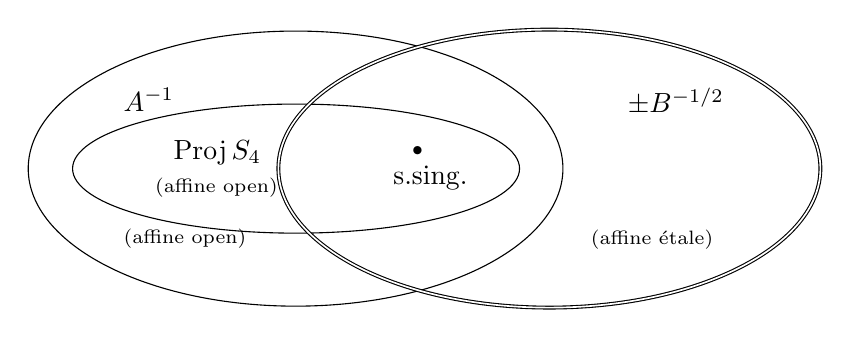
\begin{tikzpicture}[baseline=(current bounding box.center), every fit/.style={ellipse,draw,inner sep=0pt}, mytext/.style={inner sep=6pt}]
          \node[mytext,align=left,rectangle] (a) at (0, 0) {$A^{-1}$ \\ \\ \\ \\ $\scriptstyle \text{(affine open)}$}; 
          \node[mytext,align=left,rectangle] (b) at (6, 0) {$\quad~ \pm B^{-1/2}$ \\ \\ \\ \\ $\scriptstyle \text{(affine \'etale)}$}; 
          \node[mytext,align=left,rectangle] (c) at (3, 0) {$\quad~ _\bullet$ \\ ~ s.sing.}; 
          \node[mytext,align=left,rectangle] (c') at (3.2, 0) {}; 
          \node[mytext,align=left,rectangle] (d) at (.4, 0) {$~~ \Proj S_4$ \\ $\scriptstyle \text{(affine open)}$}; 
          \node[draw,fit=(a) (c)] {}; 
          \node[draw,fit=(d) (c')] {}; 
          \node[draw,double,fit=(b) (c)] {}; 
  \end{tikzpicture}
 \end{equation*}
\\
 To pass to the homotopy groups of the corresponding $E$-theory spectrum $E$, we write 
 \[
  a \ce u A, \quad h \ce u^4 H = a^4 - 16 a^2 + 26, \quad \ad \quad \d \ce u^{12} \D = h - 26 
 \]
 Following the convention that elements in algebraic degree $i$ lie in topological degree $2 i$, we then have 
 \[
  E_* \cong \BW \big( \cF_5 \big) \lb h \rb [u] 
 \]
 with $|h| = 0$ and $|u| = -2$.  
 In particular, by Hensel's lemma, the elements $a$, $\d$, and $\d^{-1}$ are all contained in $E_0$.  
 Moreover, $u$ corresponds to a coordinate on $\HCC_4$ 
 via a chosen isomorphism 
 $\Spf E^0 \BC\BP^\infty \cong \HCC_4$ of formal groups over $\Spf E^0 \cong \Spf\!\left( {S_4}^\wedge_{(5,H)} \otimes_{\BW(\BF_5)} \BW \big( \cF_5 \big) \!\right)$ (cf.~\cite[Definition 1.2]{AHS01}).  
 As an abuse of notation, recall that in Examples \ref{ex:3} and \ref{ex:4} we have written 
 \[
  u = \frac{~\!x~\!}{y} 
 \]
 where $x$ and $y$ are the affine coordinates in the Weierstrass equation for $\CC_N$; 
 the resulting algebraic degree $-1$ of $u$ matches the topological degree $-2$ of $u$ in $E_*$.  
\end{ex}
The process in the above example applies to all pairs $p$ and $N$.  
At a larger prime, the supersingular locus may contain more than one closed point, 
e.g., the Hasse invariant of $\CC_4$ at $p = 11$ factors as $(A^2 + B) (A^8 + 3 A^6 B + 4 A^2 B^3 + B^4)$.  
In this case, $H$ lifts one of the irreducible factors of the Hasse invariant.  
The corresponding closed point carries the supersingular elliptic curve whose formal group models $\BG_0 / k$ for the $E$-theory.  

\begin{rmk}
 \label{rmk:N}
 For a fixed $E$-theory, 
 the various models above each involve a choice of $N$ for the $\CP_N$-structure, 
 and a choice of an isomorphism class of supersingular elliptic curves at $p$.  
 Over a separably closed field of characteristic $p$, 
 any two formal group laws of the same height are isomorphic \cite[Th\'eor\`eme IV]{Lazard}.  
 Together with the universal property in the Lubin-Tate theorem \cite[Theorem 3.1]{LT}, 
 we see that up to isomorphism the homotopy groups of the $E$-theory are independent of the choice of a model.  
\end{rmk}

Recall that elements in $\MF\big(\G_1(N)\big)$ are functions $f$ on elliptic curves $C/R$ equipped with a $\CP_N$-structure $(P_0,\omega)$.  
Each value $f(C/R, P_0, \omega) \in R$ 
depends only on the $R$-isomorphism class of the triple $(C/R, P_0, \omega)$, 
and is subject to a modular transformation property that encodes the weight of $f$; moreover, its formation commutes with arbitrary base change 
(see, e.g., \cite[Section 1.2]{padicprop}).  
\begin{prop}
 \label{prop:mfe0}
 Let $E$ be a Morava $E$-theory of height 2 at the prime $p$.  
 There is a composite 
 \[
  \B_{p,\,N} \co \MF\big(\G_1(N)\big) \hookrightarrow E^0 \times \BZ \to E^0 
 \]
 of ring homomorphisms, 
 where the first map is injective and the second map is the projection.  
\end{prop}
\begin{proof}
 In view of Remark \ref{rmk:N}, given a model for the $E$-theory as in Example \ref{ex:mfe0}, 
 a modular form $f$ of weight $k$ maps to $\big( u^k \cdot \, f(\CC_N, P_0, du), ~ k \big) \in E^0 \times \BZ$, where $u \in \pi_{-2} E$ is the 2-periodic unit.  
 The injectivity of this map follows from the universal property of the triple $(\CC_N, P_0, du)$.  
\end{proof}

We will drop the subscripts in ``$\B_{p,\,N}$'' when there is no ambiguity.  



\section{From classical to topological Hecke operators}
\label{sec:ct}

Morava $E$-theory spectra are commutative $S$-algebras in the sense of \cite{EKMM}, and thus they come equipped with power operations.  
The work of Ando, Hopkins, and Strickland \cite{AHS04} (cf.~\cite[Theorem B]{cong}) sets up a correspondence 
between power operations on Morava $E$-theory and deformations of Frobenius isogenies of formal groups.  
At height 2, the Serre-Tate theorem \cite{LST} (cf.~\cite[Theorem 2.9.1]{KM}) sets up a second correspondence between isogenies of formal groups and isogenies of elliptic curves, in terms of their deformation theory.  

Via these two bridges, the classical action of Hecke operators on modular forms then corresponds to an action of ``topological'' Hecke operators on $E$-cohomology \cite[Section 14]{log}.  
The purpose of this section is to give an explicit comparison between these two actions.  
In particular, we will explain why the ring homomorphism $\B$ in Proposition \ref{prop:mfe0} fails to become a map of modules over a Hecke ring.  



\subsection{Isogenies and power operations}
\label{subsec:po}

Let $\CC_N$ over $S_N$ be the universal curve in Section \ref{subsec:model} for the moduli problem $\CP_N$.  
Denote by $\CG_N^{(p)}$ the universal example of a degree-$p$ subgroup of $\CC_N$.  
It is defined over an extension ring $S_N^{(p)}$ that is free of rank $p + 1$ as an $S_N$-module \cite[Theorem 6.6.1]{KM}.  
Explicitly, 
\[
 S_N^{(p)} \cong S_N[\K] / \big(W(\K)\big) 
\]
where $\K$ is a generator that satisfies $W(\K) = 0$ for a degree-$(p + 1)$ polynomial $W$ with coefficients in $S_N$.  
The roots $\K_0$, $\K_1$, \ldots, $\K_p$ of $W$ each correspond to a degree-$p$ subgroup of $\CC_N$.  
In particular, let $\K_0$ correspond to the formal component, 
whose restriction over an ordinary point is the unique degree-$p$ subgroup of $\HCC_N$.  

We write 
\[
 \Psi_N^{(p)} \co \CC_N \to \CC_N / \CG_N^{(p)} 
\]
for the universal degree-$p$ isogeny over $S_N^{(p)}$, and write $\CC_N^{(p)}$ for the quotient curve $\CC_N / \CG_N^{(p)}$.  
Following Lubin \cite[proof of Theorem 1.4]{Lubin67}, we construct $\Psi_N^{(p)}$ as a deformation of Frobenius, 
that is, over any closed point in the supersingular locus at $p$, $\Psi_N^{(p)}$ restricts as the $p$-power Frobenius endomorphism on the corresponding supersingular elliptic curve.  
\begin{cstr}[{cf.~\cite[proof of Theorem 1.4]{Lubin67} and \cite[Section 7.7]{KM}}]
 \label{cstr}
 Let $P$ be any point on $\CC_N$.  
 Write $u = x / y$ and $v = 1 / y$, 
 where $x$ and $y$ are the usual coordinates in an affine Weierstrass equation with the identity $O$ at the infinity.  
 We have $\big( u(O), v(O) \big) = (0,0)$.  
 \begin{enumerate}[(i)]
  \item  Define $\Psi_N^{(p)} \co \CC_N \to \CC_N^{(p)}$ by the formula 
  \[
   u\big(\Psi_N^{(p)}(P)\big) \ce \prod_{Q \in \CG_N^{(p)}} u(P - Q) 
  \]

  \item  Define $\K \in S_N^{(p)}$ in degree $-p + 1$ as 
  \[
   \K \ce \prod_{Q \in \CG_N^{(p)} \setminus \! \{O\}} u(Q) 
  \]
 \end{enumerate}
\end{cstr}
We verify that the isogeny $\Psi_N^{(p)}$ has kernel precisely the subgroup $\CG_N^{(p)}$.  
Moreover, it is a deformation of Frobenius, 
since at a supersingular point the $p$-divisible group is formal so that $Q = O$ for all $Q \in \CG_N^{(p)}$.  

\begin{rmk}
 \label{rmk:K}
 The element $\K$ is the ``norm'' parameter for the moduli problem $[\G_0(p)]$ as an ``open arithmetic surface'' 
 (the other parameter can be a deformation parameter coming from the Hasse invariant at $p$) \cite[Section 7.7]{KM}.  
 As $u$ is a local coordinate near the identity $O$, 
 we note that by the above construction the cotangent map $\big(\Psi_N^{(p)}\big)^*$ at $O$ sends $du$ to $\K du$.  
\end{rmk}

Via completion at a supersingular point, we see in Section \ref{subsec:mfe0} that the ring $S_N \cong \MF\big(\G_1(N)\big)$ representing $\CP_N$ is locally realized in homotopy theory as $E^0$.  
Here, given the ring $S_N^{(p)}$ representing the simultaneous moduli problem $\big(\CP_N,[\G_0(p)]\big)$, 
Strickland's theorem \cite[Theorem 1.1]{Str98} identifies the completion of $S_N^{(p)}$ as $E^0(B\Sigma_p) / I$, where $I$ is a transfer ideal.  

The universal degree-$p$ isogeny $\Psi_N^{(p)} \co \CC_N \to \CC_N^{(p)}$ 
is constructed above as a deformation of Frobenius.  
Thus by \cite[Theorem B]{cong} it corresponds to a total power operation 
\begin{equation}
 \label{psi}
 \psi^p \co E^0 \to E^0(B\Sigma_p) / I 
\end{equation}
which is independent of the choice of $N$ (see Remark \ref{rmk:N}).  
In particular, taking quotient by the transfer ideal makes this operation additive and hence a ring homomorphism.  
\begin{ex}
 \label{ex:po}
 We continue Example \ref{ex:mfe0} with $p = 5$ and $N = 4$.  

 The universal degree-$5$ isogeny $\Psi_4^{(5)} \co \CC_4 \to \CC_4^{(5)}$ is defined over the graded ring $S_4^{(5)} \cong S_4[\K] / \big(W(\K)\big)$, 
 where $|\K| = -4$ and 
 \begin{equation}
  \label{W}
  W(\K) = \K^6 - \frac{10}{B^2} \K^5 + \frac{35}{B^4} \K^4 - \frac{60}{B^6} \K^3 + \frac{55}{B^8} \K^2 - \frac{H}{B^{12}} \K + \frac{5}{B^{12}} 
 \end{equation}
 This polynomial is computed from the division polynomial $\psi_5$ in \cite[Exercise 3.7]{AEC} for the curve $\CC_4$.  
 We first deduce from $\psi_5$ identities satisfied by the $uv$-coordinates of a universal example 
 $Q \in \CG_4^{(5)} \!\setminus\!\! \{O\}$ as in \cite[proof of Proposition 2.2]{p3}.  
 We then compute an explicit formula for 
 \[
  \K = u(Q) \cdot u(-Q) \cdot u(2 Q) \cdot u(-2 Q) 
 \]
 using methods analogous to \cite[III.2.3]{AEC}.  
 Finally we solve for a monic degree-6 equation satisfied by $\K$ and obtain the polynomial $W$.  
 (We do not compute an equation for $\CC_4^{(5)}$ as in \cite[Proposition 2.3]{p3}.)  

 To pass to the corresponding power operation, write 
 \[
  \A \ce u^{-4} \K_0 
 \]
 where $\K_0$ corresponds to the formal degree-$p$ subgroup.  
 The total power operation $\psi^5 \co E^0 \to E^0(B\Sigma_5) / I$ then lands in 
 \[
  E^0(B\Sigma_5) / I \cong \BW \big( \cF_5 \big) \lb h, \A \rb / \big(w(\A)\big) 
 \]
 where $w(\A) = \A^6 - 10 \A^5 + 35 \A^4 - 60 \A^3 + 55 \A^2 - h \A + 5$.  
 To compute the effect of $\psi^5$ on the generator $h \in E^0$, we proceed as follows.  

 Consider a second universal degree-$5$ isogeny 
 \[
  \widetilde{\Psi}_4^{(5)} \co \CC_4^{(5)} \to \CC_4^{(5)} / \widetilde{\CG}_4^{(5)} 
 \]
 where $\widetilde{\CG}_4^{(5)} = \CC_4[5] / \CG_4^{(5)}$.  
 It is defined the same way as in Construction \ref{cstr}, 
 with a parameter $\widetilde{\K} \in S_4^{(5)}$ in degree $-20$.  
 Over $S_4^{(5)}$, the assignment 
 \[
  \left(\! \big( \CC_4, P_0, du \big), ~ \CG_4^{(5)} \right) \mapsto \left(\! \big( \CC_4^{(5)}, \Psi_4^{(5)}(P_0), du \big), ~ \widetilde{\CG}_4^{(5)} \right) 
 \]
 is an involution on the moduli problem $\big(\CP_4,[\G_0(5)]\big)$ (cf.~\cite[11.3.1]{KM}).  In particular, 
 by rigidity, we have the identity $\widetilde{\Psi}_4^{(5)} \circ \Psi_4^{(5)} = [5]$ that lifts from $\Frob^2 = [5]$ over the supersingular locus, 
 where $\Frob$ is the 5-power Frobenius endomorphism.  
 Thus in view of Remark \ref{rmk:K} we obtain a relation $\widetilde{\K} \cdot \K = 5 / B^{12}$ in $S_4^{(5)}$.  

 Correspondingly, in $E^0(B\Sigma_5) / I$, the relation 
 \begin{equation}
  \label{w}
  \A^6 - 10 \A^5 + 35 \A^4 - 60 \A^3 + 55 \A^2 - h \A + 5 = 0 
 \end{equation}
 gives rise to an analogous relation  
 \begin{equation}
  \label{w'}
  \widetilde{\A}^6 - 10 \widetilde{\A}^5 + 35 \widetilde{\A}^4 - 60 \widetilde{\A}^3 + 55 \widetilde{\A}^2 - \widetilde{h} \widetilde{\A} + 5 = 0 
 \end{equation}
 for quantities coming from the isogeny $\widetilde{\Psi}_4^{(5)}$, and we have 
 \begin{equation}
  \label{AA'}
  \widetilde{\A} \cdot \A = 5 
 \end{equation}
 We then compute that 
 \begin{equation}
  \label{psi5}
  \begin{split}
   \psi^5(h) = & ~ \widetilde{h} \\
             = & ~ \widetilde{\A}^5 - 10 \widetilde{\A}^4 + 35 \widetilde{\A}^3 - 60 \widetilde{\A}^2 + 55 \widetilde{\A} + \A \qquad\qquad\quad \text{by \eqref{w'} and \eqref{AA'}} \\
             = & ~ (-\A^5 + 10 \A^4 - 35 \A^3 + 60 \A^2 - 55 \A + h)^5 \\
               & - 10 (-\A^5 + 10 \A^4 - 35 \A^3 + 60 \A^2 - 55 \A + h)^4 \\
               & + 35 (-\A^5 + 10 \A^4 - 35 \A^3 + 60 \A^2 - 55 \A + h)^3 \\
               & - 60 (-\A^5 + 10 \A^4 - 35 \A^3 + 60 \A^2 - 55 \A + h)^2 \\
               & + 55 (-\A^5 + 10 \A^4 - 35 \A^3 + 60 \A^2 - 55 \A + h) \\
               & + \A \qquad\qquad\qquad\qquad\qquad\qquad\qquad\qquad\qquad\quad \text{by \eqref{AA'} and \eqref{w}} \\
             = & ~ h^5 - 10 h^4 - 1065 h^3 + 12690 h^2 + 168930 h \\
               & - 1462250 + (-55 h^4 + 850 h^3 + 39575 h^2 \\
               & - 608700 h - 1113524) \A + (60 h^4 - 775 h^3 \\
               & - 45400 h^2 + 593900 h + 2008800) \A^2 + (-35 h^4 \\
               & + 400 h^3 + 27125 h^2 - 320900 h - 1418300) \A^3 \\
               & + (10 h^4 - 105 h^3 - 7850 h^2 + 86975 h \\
               & + 445850) \A^4 + (-h^4 + 10 h^3 + 790 h^2 - 8440 h \\
               & - 46680) \A^5 \qquad\qquad\qquad\qquad\qquad\qquad\qquad\quad~~~ \text{by \eqref{w}} 
  \end{split}
 \end{equation}
 The assignment $(h, \A) \mapsto (\widetilde{h}, \widetilde{\A})$ is an involution on $E^0(B\Sigma_5) / I$ 
 that corresponds to the Atkin-Lehner involution of modular forms on $\G_0(5)$ (cf.~\cite[Lemmas 7--10]{AtkinLehner} and \cite[11.3.1]{KM}).  
\end{ex}
The previous example illustrates a general recipe for computing power operations on Morava $E$-theory at height 2 and prime $p$, 
with a model based on the moduli problem $\big(\CP_N,[\G_0(p)]\big)$.  
Crucial in this computation is an explicit form for 
\begin{equation}
 \label{generalw}
 w(\A) = \A^{p + 1} + w_p \A^p + \cdots + w_1 \A + w_0 \in E^0[\A] 
\end{equation}
The coefficients have the following properties.  
\begin{itemize}
 \item For $i \neq 1$, each $w_i$ is divisible by $p$.  

 \item The coefficient $w_1$ is a lift of the Hasse invariant at $p$, 
 so we can always choose $h = -w_1$ and have $w(\A) \equiv \A (\A^p - h) \mod p$.  

 \item We have $w_0 = \widetilde{\A} \cdot \A = \mu p$ for some unit $\mu \in E^0$ depending on the Frobenius endomorphism of the supersingular curve 
 (cf.~\cite[3.8]{mc1}).  
\end{itemize}
Computing $w(\A)$ appears to be essentially computing a ``modular equation'' (see, e.g., \cite[II.6]{Milne} and \cite{MO}).  

\begin{rmk}
 \label{rmk:invl}
 It does not work in general to compute $\psi^p(h)$ based solely on the involution of $w(\A)$ and the relation 
 \begin{equation}
  \label{w0}
  \widetilde{\A} \cdot \A = w_0 
 \end{equation}
 The coefficients $w_i$, $2 \leq i \leq p$, may involve $h$ (in terms of functions of $a$).  
 For example, using $\CP_3$ instead of $\CP_4$ for the prime 5, we have 
 \[
  w(\A) = \A^6 - 5 a \A^4 + 40 \A^3 - 5 a^2 \A^2 - h \A - 5 
 \]
 with $h = -a^4 + 19 a$.  
 In this case, it seems unavoidable to compute an explicit equation for the quotient curve $\CC_N^{(p)}$ 
 (see, e.g., \cite[proof of Proposition 2.3]{p3}).  
\end{rmk}



\subsection{Hecke operators}
\label{subsec:ho}

We first describe the classical action of Hecke operators on modular forms in terms of isogenies between elliptic curves.  
The $p$'th Hecke operator $T_p$ that acts on $\MF\big(\G_1(N)\big)$ can be built from universal isogenies as follows.  
\begin{cstr}[{cf.~\cite[(1.11.0.2)]{padicprop}}]
 \label{cstr:Tp}
 Let the notation be as in Section \ref{subsec:po}, with the subscripts ``$N$'' suppressed.  
 Given any $f \in \MF\big(\G_1(N)\big)$ of weight $k \geq 2$, $T_p~f \in \MF\big(\G_1(N)\big)$ is a modular form such that 
 \begin{equation}
  \label{Tp}
  T_p~f(\CC_S, P_0, du) \ce \frac{1}{p} \sum_{i=0}^p \K_i^k \cdot f\!\left(\CC_{S^{(p)}}/\CG^{(p)}_i, \Psi^{(p)}_i(P_0), du\right) 
 \end{equation}
 where each $\CG^{(p)}_i$ denotes a degree-$p$ subgroup, and $\Psi^{(p)}_i$ is the corresponding quotient map.  
\end{cstr}
\begin{rmk}
 \label{rmk:normalizing}
 The terms $\K_i^k$ appear in the above formula so that $T_p$ is independent of the choice of a basis for the cotangent space.  
 Explicitly, we have 
 \[
  \big( \Psi^{(p)}_i \big)^* du = \K_i \cdot du \qquad \ad \qquad \big( \Psi^{(p)}_i \big)^* \big( \widecheck{\Psi}^{(p)}_i \big)^* du = p \cdot du 
 \]
 where each $\widecheck{\Psi}^{(p)}_i \co \CC/\CG^{(p)}_i \to \CC$ is a dual isogeny, 
 and $\big( \widecheck{\Psi}^{(p)}_i \big)^* du$ is the choice in \cite{padicprop} for a nowhere-vanishing one-form on a quotient curve 
 (cf.~Remark \ref{rmk:K} and [ibid., discussion before (1.11.0.0) in Section 1.11]).  
 Thus we can rewrite \eqref{Tp} as 
 \begin{equation*}
  \begin{split}
     & ~ \frac{1}{p} \sum_{i=0}^p \K_i^k \cdot f\!\left(\CC_{S^{(p)}}/\CG^{(p)}_i, \Psi^{(p)}_i(P_0), du\right) \\
   = & ~ \frac{1}{p} \sum_{i=0}^p \K_i^k \cdot f\!\left(\CC_{S^{(p)}}/\CG^{(p)}_i, \Psi^{(p)}_i(P_0), (\K_i/p) \big(\widecheck{\Psi}^{(p)}\big)^* du\right) \\
   = & ~ \frac{1}{p} \sum_{i=0}^p p^k \cdot f\!\left(\CC_{S^{(p)}}/\CG^{(p)}_i, \Psi^{(p)}_i(P_0), \big(\widecheck{\Psi}^{(p)}\big)^* du\right) 
  \end{split}
 \end{equation*}
 and this agrees with [ibid., (1.11.0.2)].  
\end{rmk}

\begin{cstr}[{cf.~\cite[1.12]{log}}]
 \label{cstr:tp}
 There is a topological Hecke operator $t_p \co E^0 \to p^{-1} E^0$ defined by 
 \begin{equation}
  \label{tp}
  t_p(x) \ce \frac{1}{p} \sum_{i=0}^p \psi^p_i(x) 
 \end{equation}
 where $\psi^p_i$ denotes the power operation $\psi^p \co E^0 \to E^0(B\Sigma_p) / I \cong E^0[\A] / \big( w(\A) \big)$ with the parameter $\A$ replaced by $\A_i = u^{-p + 1} \K_i$.  
\end{cstr}
Since the parameters $\A_i$ are the roots of the polynomial $w \in E^0[\A]$, 
$t_p$ indeed lands in $p^{-1} E^0$.  
\begin{rmk}
 \label{rmk:tc}
 The topological Hecke operator above does not coincide with the classical one on modular forms via the ring homomorphism $\B$ in Proposition \ref{prop:mfe0}.  
 Comparing \eqref{tp} to \eqref{Tp}, note that there are no terms $\A_i^k$ corresponding to $\K_i^k$.  
 This is related to the fact that the map $\B$ is not injective: 
 if we include $\A_i^k$ in the definition, for each $x \in E^0$ we need to determine a unique value of its ``weight'' $k$ so that $t_p$ is well-defined.  

 Note that the map $\B$ is not surjective either, so an element in $E^0$ may not come from any modular form.  
 On the other hand, the total power operation $\psi^p$ is defined on the entire ring $E^0 \cong \BW \big( \cF_p \big) \lb h \rb$.  
 In particular, a formula for $\psi^p(h)$ extends by continuity to give $\psi^p(x)$ for any $x \in E^0$, as $\psi^p$ is a ring homomorphism 
 ($\psi^p(c) = F c$ for $c \in \BW \big( \cF_p \big)$, with $F$ the Frobenius automorphism).  
\end{rmk}
\begin{ex}
 \label{ex:ho}
 Again, let $p = 5$ and $N = 4$.  
 Recall from Example \ref{ex:mfe0} that we have 
 \[
  \B(\D) = \d = h - 26 
 \]
 In view of \eqref{w}, we then compute from \eqref{psi5} that 
 \begin{equation*}
  \begin{split}
   t_5(\d) = & ~ \frac{1}{5} \sum_{i=0}^5 \psi^5_i(\d) \\
           = & ~ \frac{1}{5} \sum_{i=0}^5 \big(\psi^5_i(h) - 26\big) \\
           = & ~ \frac{1}{5} (h^5 - 10 h^4 - 1340 h^3 + 18440 h^2 + 267430 h - 3178396) \\
           = & ~ \frac{1}{5} (h^4 + 16 h^3 - 924 h^2 - 5584 h + 122246) \cdot \d 
  \end{split}
 \end{equation*}
 Given that the modular form $\D$ is of weight 12, we define and compute 
 \begin{equation*}
  \begin{split}
   \overline{t}_5(\d) \ce & ~ \frac{1}{5} \sum_{i=0}^5 \A_i^{12} \cdot \psi^5_i(\d) \qquad\qquad\qquad\qquad\qquad\qquad\qquad\qquad\quad \\
                        = & ~ 4830 h - 125580 \\
                        = & ~ \T(5) \cdot \d 
  \end{split}
 \end{equation*}
 where $\T \co \BN \to \BZ$ is the Ramanujan tau-function, with $\T(5) = 4830$.  
 This recovers the action of $T_5$ on $\D$.  
\end{ex}

More generally, in the theory of automorphic forms for $\G_1(N) \subset \SL_n(\BZ)$, 
the above Hecke operator $T_p$ can be renamed as $T_{1,\,p}$.  
It belongs to a family of operators $T_{i,\,p}$, $1 \leq i \leq n$ 
that generate the $p$-primary Hecke ring (see, e.g., \cite[Theorem 3.20]{AF}).  

For the case $n = 2$, the other Hecke operator $T_{2,\,p}$ arises from the isogeny of multiplication by $p$, whose kernel is the degree-$p^2$ subgroup consisting of the $p$-torsion points.  
Explicitly (again with ``$N$'' suppressed), given any $f \in \MF\big(\G_1(N)\big)$ of weight $k \geq 2$, 
\begin{equation}
 \label{T2p}
 \begin{split}
  T_{2,\,p}~f(\CC_S, P_0, du) \ce & ~ \frac{1}{p^2} \Big(\! \big( p B^{-(p - 1)(p + 1)/|B|} \big)^k \!\cdot f\!\left(\CC_{S^{(p)}}/\CC[p], p P_0, du\right) \!\!\Big) \\
                                = & ~ p^{k - 2} \!\cdot f(\CC_S, P_0, du) 
 \end{split}
\end{equation}
Here the factor $B^{-(p - 1)(p + 1)/|B|}$ arises from the $S^{(p)}$-isomorphism 
\begin{equation}
 \label{iso}
 \CC/\CC[p] \cong \frac{\CC/\CG^{(p)}}{\CC[p]/\CG^{(p)}} = \frac{\CC^{(p)}}{\widetilde{\CG}^{(p)}} 
\end{equation}
where the last group scheme is the target of the composite $\widetilde{\Psi}^{(p)} \circ \Psi^{(p)}$ of Frobenius isogenies.  

Topologically, given any $K(2)$-local commutative $E$-algebra $A$, 
there is a composite $\f$ of total power operations $\psi^p \circ \psi^p \co A^0 \to A^0$.  
Note that $\phi$ lands in $A^0$, 
because up to the isomorphism \eqref{iso} the composite $\widetilde{\Psi}^{(p)} \circ \Psi^{(p)}$ is an endomorphism on $\CC$ over $S$.  
In particular, on $E^0$ or on $E^0(B\Sigma_p) / I$, the operation 
$\phi$ is the identity map, which is a manifest of the Atkin-Lehner involution (see the end of Example \ref{ex:po}).  

We define the topological Hecke operator $t_{2,\,p} \co E^0 \to p^{-1} E^0$ by 
\begin{equation}
 \label{t2p}
 t_{2,\,p}(x) \ce p^{-2} \phi(x) 
\end{equation}
Write $t_{1,\,p} \ce t_p$.  
The ring $\BZ[t_{1,\,p},t_{2,\,p}]$ then acts on $p^{-1} E^0$.  
As we see in Remark \ref{rmk:tc}, along the map $\B \co \MF\big(\G_1(N)\big) \to E^0$, 
this action is not compatible with the action of the Hecke ring $\BZ[T_{1,\,p},T_{2,\,p}]$ on the subring of $\MF\big(\G_1(N)\big)$ consisting of elements of weight $k \geq 2$.  
However, in certain instances, the two actions do interact well.  
The next section will exploit this connection.  



\section{Kernels of logarithmic cohomology operations at height 2}
\label{sec:kerlog}

Section \ref{subsec:ho} gives an explicitation of a ring of topological Hecke operators acting on $E^0$, where $E$ is a Morava $E$-theory of height 2.  
Based on this, we now use a number-theoretic calculation to understand a topological construction.  
This is Rezk's construction of logarithmic cohomology operations \cite{log}.  
We first recall a formula of Rezk for computing these operations, which leads to a connection with Hecke operators.  



\subsection{Connecting to Hecke operators}

Given any commutative $S$-algebra $R$, 
Rezk constructs a family of operations that naturally acts on the spectrum of units of $R$ \cite[Definition 3.6]{log}.  
Specifically, given a positive integer $n$ and a prime $p$, consider the composite 
\begin{equation}
 \label{log}
 \gl_1 R \to L_{K(n)} \gl_1 R \simeq \Phi_n \Omega^\infty \gl_1 R \xrightarrow{\sim} \Phi_n \Omega^\infty R \simeq L_{K(n)} R 
\end{equation}
where $\gl_1 R$ is the units spectrum, $L_{K(n)}$ denotes localization with respect to the $n$'th Morava $K$-theory at $p$, 
and $\Phi_n$ is the corresponding Bousfield-Kuhn functor from the category of based topological spaces to the category of spectra.  
Note that the spaces $\Omega^\infty \gl_1 R$ and $\Omega^\infty R$ have weakly equivalent basepoint components, 
but the standard inclusion $\Omega^\infty \gl_1 R \hookrightarrow \Omega^\infty R$ is not basepoint-preserving.  
The equivalence $\Phi_n \Omega^\infty \gl_1 R \to \Phi_n \Omega^\infty R$ thus involves a ``basepoint shift'' [ibid., 3.4].  

Let $E$ be a Morava $E$-theory at height $n$ and prime $p$.  
With $R = E$, the target of \eqref{log} represents completed $E$-homology 
$E^{\scriptscriptstyle \wedge}_*(-) \ce \pi_* L_{K(n)}(E \wedge -)$, 
which is $E^0$-linear dual to $E$-cohomology.  
Applying $\pi_0(-)$ to \eqref{log}, we then obtain the logarithmic operation 
\[
 \ell_{n,\,p} \co \big( E^0 \big)^{\!\times} \to E^0 
\]
which is a homomorphism from a multiplicative group to an additive group.  
More generally, taking $R$ to be the spectrum of functions from $\Sigma^\infty_+ X$ to $E$ for a space $X$, 
it acts on $E^0(X)^\times$, naturally both in $X$ and in $E$.  

The main theorem of \cite{log} is a formula for this operation [ibid., Theorem 1.11].  
In particular, for any $x \in \big( E^0 \big)^{\!\times}$, 
\[
 \ell_{n,\,p}(x) = \frac{1}{p} \log\big(1 + p M(x)\big) 
\]
where $M \co \big( E^0 \big)^{\!\times} \to E^0$ is a cohomology operation 
that can be expressed in terms of power operations $\psi_A$ associated to certain subgroups $A$ of $(\BQ_p/\BZ_p)^n$.  
Explicitly, 
\[
 1 + p M(x) = \prod_{j=0}^n \prod_{\stackrel{\scriptstyle A \subset (\BQ_p/\BZ_p)^n [p]}{\#A = p^j}} \psi_A(x)^{(-1)^j p^{(j-1)(j-2)/2}} 
\]

Now let the $E$-theory be of height $n = 2$.  
In the presence of a model for $E$, the operations $\psi_A$ above coincide with the power operations discussed in Section \ref{sec:ct}.  
In particular, 
\begin{equation}
 \label{l2p}
 \ell_{2,\,p}(x) = \frac{1}{p} \log \left( x^p \cdot \frac{1}{\psi^p_0(x) \cdots \psi^p_p(x)} \cdot \phi(x) \right) 
\end{equation}
Note that $\ell_{2,\,p}(x) = 0$ for any $x \in \BZ \cap \big( E^0 \big)^{\!\times}$.  

Suppose that $x = \B(\,f)$ for some modular form $f$ of weight $k$ (see Proposition \ref{prop:mfe0}).  
We next write \eqref{l2p} in terms of Hecke operators.  
We note the following.  
\begin{itemize}
 \item Recall from \eqref{generalw} that the parameters $\A_i$ in the operations $\psi^p_i$ satisfy 
 \[
  \A_0 \cdots \A_p = (-1)^{p+1} w_0 = (-1)^{p+1} \mu p 
 \]
 for some $\mu \in \big( E^0 \big)^{\!\times}$.  
 Even better, by a theorem of Ando \cite[Theorem 4]{Ando95}, there exists a unique coordinate on the formal group of $E$ such that 
 its corresponding parameters $\A_i$ satisfy $\A_0 \cdots \A_p = p$.  
 This is the coordinate $u = x/y$ when $p = 2$ with the $\CP_3$-model \cite[Section 3]{h2p2} 
 and when $p = 5$ with the $\CP_4$-model \eqref{w}.  
 Henceforth we will choose this particular coordinate for all primes $p$.  

 \item Recall that $\psi^p_i$, $\phi$ and $\B$ are ring homomorphisms.  
 Multiplication by the terms $\K_i^k$ in \eqref{Tp} and by $p^k$ in \eqref{T2p} can be viewed as ring homomorphisms as well.  
 More precisely, we allow the exponent $k$ to vary, 
 according to the weight of the modular form that immediately follows.  
 We will denote these ring homomorphisms by $\K_i^\bullet$ and $p^\bullet$.  
 The topological analog of $\K_i^\bullet$ on homotopy groups is $\A_i^\bullet$.  
\end{itemize}
In Section \ref{subsec:ho} we give a comparison between classical and topological Hecke operators, particularly as illustrated in Example \ref{ex:ho}.  
In view of this comparison and the two observations above, we can now rewrite \eqref{l2p} as follows (cf.~\cite[1.12]{log}).  
Given $x = \B(\,f)$, 
\begin{equation}
 \label{grdl2p}
 \begin{split}
  \ell_{2,\,p}(x) = & ~ \frac{1}{p} \log \frac{x^p \cdot p^\bullet \phi(x)}{\prod_{i=0}^p \A_i^\bullet \psi^p_i(x)} \\
                 = & \left( 1 - \frac{1}{p} \sum_{i=0}^p \A_i^\bullet \psi^p_i + p \cdot \frac{1}{p^2} p^\bullet \phi \right) \log x \\
                 = & ~ \B \left( (1 - T_{1,\,p} + p \cdot T_{2,\,p}) \log f \right) 
 \end{split}
\end{equation}
Following Rezk loc.~cit., we write 
\begin{equation}
 \label{FX}
 F_X \ce 1 - T_{1,\,p} \cdot X + p T_{2,\,p} \cdot X^2 \in \BZ[T_{1,\,p},T_{2,\,p}][X] 
\end{equation}
In particular, with $X = 1$, \eqref{grdl2p} becomes 
\begin{equation}
 \label{F1}
 \ell_{2,\,p}(x) = \B \big( F_1 (\log f) \big) 
\end{equation}

\begin{rmk}
 \label{rmk:ratio}
 Let $x = \B(\,f) \in \big( E^0 \big)^{\!\times}$ for some unit 
 $f$ in $\MF\big(\G_1(N)\big)$ of weight $k$ (cf.~\cite{KubertLang}).  
 The formula \eqref{l2p} expresses $p \ell_{2,\,p}(x)$ as the logarithm of a ratio: 
 the numerator, via $\B$, corresponds to a modular form of weight $p k + p^2 k$, 
 and the denominator corresponds to one having weight $(p + 1) p k = p k + p^2 k$.  
 Thus $p \ell_{2,\,p}(x)$ corresponds to a $p$-adic modular form of weight 0 (cf.~\cite[Section 10.1]{padicinterp}).  
 We note the similarity between the logarithms loc.~cit.~and the formula in \cite[Theorem 1.11]{log}; 
 in particular, compare the logarithm in \cite[10.2.7]{padicinterp} and the case $n = 1$ as in \cite[Theorem 1.9]{log}.  
\end{rmk}

\begin{ex}
 \label{ex:log}
 We revisit the case $p = 5$, with the model for the $E$-theory given by the moduli problem $\CP_4$.  
 Consider $\d = \B(\D) \in \big( E^0 \big)^{\!\times}$.  
 As in Example \ref{ex:ho}, we calculate from \eqref{psi5} and \eqref{w} that 
 \begin{equation*}
  \begin{split}
   \ell_{2,\,5}(\d) = & ~ \frac{1}{5} \log \left( \d^5 \cdot \frac{1}{\psi^p_0(\d) \cdots \psi^p_p(\d)} \cdot \phi(\d) \right) \\
                  = & ~ \frac{1}{5} \log \left( \d^5 \cdot \frac{1}{\d^6} \cdot \d \right) \\
                  = & ~ \frac{1}{5} \log 1 \\
                  = & ~ 0 
  \end{split}
 \end{equation*}
 We compare this to the prime-2 case with the $\CP_3$-model.  
 In \cite[2.8]{h2p2}, Rezk computes that 
 \[
  \ell_{2,\,2}\big(\B(\D)\big) = \frac{1}{2} \log(-1) 
 \]
 Interpreting the ``$\log$'' here as the 2-adic logarithm (see, e.g., \cite[\S IV.1]{padic} and cf.~\cite[10.2.16]{padicinterp}), 
 we get a second example where the modular form $\D$ produces an element in the kernel of $\ell_{2,\,p}$.  

 Moreover, for the prime-2 case, recall from Example \ref{ex:3} that $\D = B^3 (A^3 - 27 B)$.  
 Thus 
 \[
  \B(\D) = (a - 3) (a^2 + 3 a + 9) 
 \]
 with $E^0 \cong \BW \big( \cF_2 \big) \lb a \rb$ (cf.~\cite[Section 4]{h2p2}).  
 Using Rezk's formula for the total power operation on $E^0$, we compute that 
 \[
  \ell_{2,\,2}(a - 3) = \frac{1}{2} \log(-1) = 0 
 \]
 \[
  \ell_{2,\,2}(a^2 + 3 a + 9) = \frac{1}{2} \log 1 = 0 
 \]
 Thus, as $\ell_{2,\,2}$ is a group homomorphism, the formal power series 
 \[
  \frac{1}{a - 3} = -\sum_{i = 0}^\infty \Big( \sum_{j = 0}^\infty (-2)^j \Big)^{i + 1} a^i ~ \in \BW \big( \cF_2 \big) \lb a \rb^\times 
 \]
 is also contained in the kernel of $\ell_{2,\,2}$.  

 The above turn out to be instances of a general vanishing result for the logarithms that we discuss next.  
\end{ex}



\subsection{Detecting the kernels}
\label{subsec:thm}

In this section, via the formula \eqref{grdl2p} for the logarithmic operation in terms of Hecke operators, we 
detect a family of elements contained in the kernel of this operation.  
It includes the elements computed in Example \ref{ex:log}.  
Roughly speaking, any modular form with vanishing Serre derivative gives an element in the kernel.  

We first review some preliminaries about differential structures on rings of modular forms 
(see, e.g., \cite[Section 5 of Part 1]{1-2-3} and \cite[Section 2.3]{web}).  
In connection to Morava $E$-theories, 
we have been considering the $p$-local behavior of integral modular forms of level $N$, 
with $p$ not dividing $N$ 
(which embed into the ring of $p$-adic modular forms).  
Thus for our purpose these modular forms can equivalently be viewed as over $\BC$.  
Henceforth we will freely interchange between these two perspectives.  

Recall that there is a differential operator $D$ acting on meromorphic elliptic functions over $\BC$.  
Specifically, given any meromorphic modular form $f$, it has a $q$-expansion 
\[
 f(z) = \sum_{j > -\infty} a_j q^j 
\]
with $a_j \in \BC$.  
(This is indeed $f$ evaluated at the pair $\big(\Tate(q) / \BZ \lp q \rp, \o_\can\big)$, 
where $\Tate(q)$ is the Tate curve and $\o_\can$ is the canonical nowhere-vanishing invariant one-form on it.)  
We then have 
\begin{equation}
 \label{ramanujan}
 D ~\! f \ce \frac{1}{2 \pi i} \frac{df}{dz} = q \frac{df}{dq} 
\end{equation}
If the $q$-expansion of $f$ has coefficients in $\BZ$, so does the $q$-series for $D ~\! f$.  

In general, the function $D ~\! f$ is no longer modular.  
There is another derivation $\vartheta$ that preserves modularity.  
If $f$ has weight $k$, its {\em Serre derivative} is given by 
\begin{equation}
 \label{serre}
 \vartheta ~\! f \ce D ~\! f - \frac{k}{12} \CE_2 \cdot f 
\end{equation}
where $\CE_2$ is the quasimodular Eisenstein series of weight 2.  
This defines a meromorphic modular form of weight $k + 2$ (see [ibid., Proposition 2.11] and cf.~\cite[Th\'eor\`eme 5(a)]{fmpadiq}).  

\begin{thm}
 \label{thm:kerlog}
 Let $E$ be a Morava $E$-theory of height 2 at the prime $p$, and let $N > 2$ be any integer prime to $p$.  
 Let 
 \[
  \ell_{2,\,p} \co \big( E^0 \big)^{\!\times} \to E^0 
 \]
 be Rezk's logarithmic cohomology operation.  
 Let 
 \[
  \B \co \MF\big(\G_1(N)\big) \to E^0 
 \]
 be the ring homomorphism in Proposition \ref{prop:mfe0}.  
 Suppose that \, $f \in \MF\big(\G_1(N)\big)^{\!\times}$ has $q$-expansion $\sum_{j = m}^\infty a_j q^j$ with $a_m = 1$.  
 If the Serre derivative $\vartheta ~\! f = 0$, then 
 the element $\B(\,f)$ is contained in the kernel of $\ell_{2,\,p}$.  
\end{thm}
Our proof consists in two parts.  
The first part (Lemma \ref{lem:const} below) shows that $\ell_{2,\,p}\big(\B(\,f)\big)$ is ``constant'' in the sense that it is the image of a constant modular form under $\B$.  
This is based on an interplay between the differential structure and the action of Hecke operators on modular forms.  
Looking at $q$-expansions, the second part then shows that this constant equals zero, which boils down to an analysis of the behavior of Tate curves under isogenies.  

\begin{lem}
 \label{lem:const}
 Given any $f \in \MF\big(\G_1(N)\big)^{\!\times}$ such that $\vartheta ~\! f = 0$, the elliptic function $F_1(\log f)$ is constant, 
 where $F_1 = 1 - T_{1,\,p} + p T_{2,\,p}$ is the operator defined in \eqref{FX}.  
\end{lem}
\begin{proof}
 Suppose that $f$ is of weight $k$.  
 By \eqref{serre}, since $\vartheta ~\! f = 0$, we have 
 \[
  D \log f = \frac{D ~\! f}{f} = \frac{k \CE_2}{12} 
 \]
 Note that $\CE_2$ is a weight-2 eigenform for every Hecke operator $T_m = T_{1,\,m}$, $m \geq 1$ with eigenvalue $\si_1(m)$.  

 By comparing the effects on $q$-expansions, we have 
 \begin{equation}
  \label{DT}
  D \circ T_{i,\,p} = \frac{1}{p^i} \cdot T_{i,\,p} \circ D 
 \end{equation}
 for $i = 1$ and $i = 2$ (cf.~\cite[Remarque after Th\'eor\`em 5]{fmpadiq}).  
 We then compute that 
 \begin{equation*}
  \begin{split}
   D \big( F_1(\log f) \big) = & ~ D \big( (1 - T_{1,\,p} + p T_{2,\,p}) \log f \big) \\
                             = & \left( 1 - \frac{1}{p} \cdot T_{1,\,p} + \frac{1}{p^2} \cdot p T_{2,\,p} \right) (D \log f) \\
                             = & \left( 1 - \frac{1}{p} \cdot T_{1,\,p} + \frac{1}{p^2} \cdot p T_{2,\,p} \right) \frac{k \CE_2}{12} \\
                             = & \left( 1 - \frac{1}{p} \cdot (1 + p) + \frac{1}{p^2} \cdot p \Big( \frac{1}{p^2} \cdot p^2 \Big) \!\! \right) \frac{k \CE_2}{12} \\
                             = & ~ 0 
  \end{split}
 \end{equation*}
 Thus as a function of the complex variable $z$, $F_1(\log f)$ is constant.  
\end{proof}

\begin{proof}[Proof of Theorem \ref{thm:kerlog}]
 Let $x \ce \B(\,f)$.  Since $\B$ is a ring homomorphism, $x \in \big( E^0 \big)^{\!\times}$.  
 Recall from \eqref{grdl2p} that 
 \begin{equation}
  \label{grdl2pbis}
  \ell_{2,\,p}(x) = \frac{1}{p} \log \frac{x^p \cdot p^\bullet \phi(x)}{\prod_{i=0}^p \A_i^\bullet \psi^p_i(x)} = \B \big( F_1(\log f) \big) 
 \end{equation}
 By Lemma \ref{lem:const}, the above is a constant in $\BW \big( \cF_p \big)^{\!\times}$, which we denote by $c_f$.  

 Suppose that $f$ has weight $k$.  
 Via the correspondence between power operations and deformations of Frobenius in \cite[Theorem B]{cong}, 
 the ratio of values of power operations on $x$ in \eqref{grdl2pbis} 
 equals a ratio of values of $f$ on the corresponding universal elliptic curves.  
 Explicitly, with notation as in \eqref{Tp} and \eqref{T2p}, we have 
 \begin{equation}
  \label{ratio}
  \frac{x^p \cdot p^\bullet \phi(x)}{\prod_{i=0}^p \A_i^\bullet \psi^p_i(x)} = 
  \frac{f(\CC_S, P_0, du)^p \cdot p^k f(\CC_S, P_0, du)}
  {\prod_{i=0}^p \K_i^k ~ f\!\big(\CC_{S^{(p)}}/\CG^{(p)}_i, \Psi^{(p)}_i(P_0), du\big)} 
 \end{equation}
 To determine the constant $c_f$, we need only inspect the constant term in the $q$-expansion for the right-hand side 
 at the cusp corresponding to the $\G_1(N)$-structure $P_0$.  

 In a formal neighborhood of the cusp, 
 the universal curve $\CC$ is isomorphic to the Tate curve $\Tate(q^N)$ over $\BZ [1/N] \lp q \rp$.  
 The universal degree-$p$ isogeny is defined over the extension ring $\BZ [1/pN, \zeta_p] \lp q^{1/p} \rp$, 
 where $\zeta_p$ is a primitive $p$'th root of unity (see \cite[Sections 1.2, 1.4, and 1.11]{padicprop}).  
 In particular, the $(p + 1)$ subgroups of order $p$ are 
 \[
  \qquad~~ \text{$G^{(p)}_0$,~~~generated by $\zeta_p$,} \qquad \ad \qquad \text{$G^{(p)}_i$, $1 \leq i \leq p$,~~~generated by $(\zeta_p^i q^{1/p})^N$} 
 \]
 We now compare as follows the lowest powers of $q$ at the denominator and the numerator of \eqref{ratio}.  

 By [ibid., (1.11.0.3) and (1.11.0.4)], including a normalizing factor $p^k$ in place of $\K_i^k$ (see Remark \ref{rmk:normalizing}), 
 we have at the denominator a leading term as the product of 
 \[
  p^k (q^p)^m \qquad \ad \qquad p^k \left( p^{-k} \zeta_p^i \big( q^{1/p} \big)^m \right) 
 \]
 where $i$ runs from 1 to $p$.  

 At the numerator, for the first factor, we have a leading term $(q^m)^p$.  
 For the second factor, we have a leading term $p^k q^m$.  

 Putting the above together, we see that the ratio has a leading constant term 
 \[
  \frac{(q^m)^p \cdot p^k q^m}{p^k (q^p)^m \cdot \prod_{i=1}^p p^k \Big( p^{-k} \big( \zeta_p^i q^{1/p} \big)^m \Big)} = \zeta_p^{-m (1 + p) p / 2} = \left\{\!\!
  \begin{array}{ll}
    (-1)^m & \quad \text{if $p = 2$} \\
    1 & \quad \text{if $p$ is odd} 
  \end{array}
  \right.
\]
Thus applying the $p$-adic logarithm (cf.~Example \ref{ex:log}) we get $c_f = 0$.  
\end{proof}

\begin{rmk}
 \label{rmk:kertheta}
 For any meromorphic modular form $f$ on $\SL_2(\BZ)$, 
 Bruinier, Kohnen, and Ono give an explicit formula for $\vartheta ~\! f$ as a multiple of $f$ by a certain function $f_\Theta$ \cite[Theorem 1]{BKO}.  
 This function $f_\Theta$ encodes a family of modular functions $j_m(z)$, $m \geq 0$, defined by applying Hecke operators to the usual $j$-invariant, 
 whose values are of arithmetic and combinatorial significance.  

 In particular, the formula of Bruinier, Kohnen, and Ono immediately shows 
 that $f$ has vanishing Serre derivative 
 precisely when its zeros and poles, if any, are located only at the cusp 
 (cf.~\cite[Proposition 6]{DumasRoyer}).  
 The functions in Example \ref{ex:log}, and in fact any unit in $\MF\big(\G_1(N)\big)$, all have the latter property, 
 though they are associated to $\G_1(N)$ instead of $\SL_2(\BZ)$ 
 (cf.~\cite[Remark 2.17]{web}).  
\end{rmk}



\section{Extending the action of Hecke operators onto logarithmic $q$-series}
\label{sec:logq}

The purpose of this section is to give an account of elliptic functions of the form $\log f$, 
where $f$ is a meromorphic modular form.  
As we have seen in Section \ref{sec:kerlog}, such functions arise in computations 
for logarithmic cohomology operations on Morava $E$-theories at height 2, e.g., in \eqref{grdl2p}.  
\begin{ex}
 \label{ex:logD}
 Let $\D$ be the modular discriminant, a cusp form of weight 12.  
 Consider the function $\log \D$.  
 The product expansion 
 \[
  \D = q \prod_{n=1}^\infty (1 - q^n)^{24} 
 \]
 implies that 
 \begin{equation}
  \label{logD}
  \begin{split}
   \log \D = & ~ \log q + 24 \sum_{n=1}^\infty \log(1 - q^n) \\
           = & ~ \log q - 24 \sum_{m=1}^\infty \si_{-1}(m) q^m 
  \end{split}
 \end{equation}
 The second summand is a usual $q$-series; 
 up to a normalization, we may call it the {\em Eisenstein series of weight $0$}, 
 by analogy to $q$-expansions for the usual Eisenstein series of higher weight 
 (also cf.~the real analytic Eisenstein series of weight 0 discussed in \cite[Sections 3.3 and 4.1]{Funke}).  

 The first summand, $\log q$, never shows up in the $q$-expansion of a meromorphic modular form.  
 It is indeed this term that we will address, 
 given the importance of $\D$ in the context of logarithmic operations (see Theorem \ref{thm:kerlog}).  
 Specifically, with motivations from homotopy theory, 
 we aim to extend the classical action of Hecke operators on $q$-series to incorporate examples such as \eqref{logD}.  
 We will then apply this to Theorem \ref{thm:kerlog} in Example \ref{ex:pf}.  
\end{ex}

In \cite{KnoppMason}, given a representation $\rho \co \SL_2(\BZ) \to \GL_n(\BC)$, 
Knopp and Mason consider $n$-dimensional vector-valued modular forms associated to $\rho$.  
In particular, they show in [ibid., Theorem 2.2 (cf.~(7) and (13))] that the components of certain vector-valued modular forms are functions 
\begin{equation}
 \label{logq}
 f(z) = \sum_{j=0}^t (\log q)^j ~\! h_j(z) 
\end{equation}
where $t \geq 0$ is an integer, and each $h_j$ is a $q$-series with at worst real exponents.  
They point out that $q$-expansions of this form occur in logarithmic conformal field theory 
(e.g., cf.~\cite[(5.3.9)]{Zhu} and \cite[Proposition 4.5]{Miyamoto}).  
The one in \eqref{logD} gives another example.  
Following Knopp and Mason, we call the series in \eqref{logq} a {\em logarithmic $q$-series}.  

\begin{prop}
 \label{prop:logq}
 Given any prime $p$, the action of the Hecke operator $T_p$ on $q$-expansions of modular forms extends so that 
 \[
  T_p (\log q) = \big( p^{-1} + p^{-2} \big) \log q 
 \]
\end{prop}
\begin{proof}
 Let $N > 2$ be an integer prime to $p$.  
 We follow the modular description in \cite[Section 1.11]{padicprop} for Hecke operators in the presence of the Tate curve 
 $\Tate(q^N)$ over $\BZ \lp q^{1 / p} \rp \otimes_\BZ \BZ [1 / p N, \zeta_p]$, where $\zeta_p$ is a primitive $p$'th root of unity.  

 Write $\CF \ce \log q$.  
 Notation as in [ibid., Section 1.2], let $\o_\can$ be the canonical nowhere-vanishing invariant one-form on $\Tate(q^N)$.  
 Let $\CM_N \ce \Proj S_N$ be the scheme over $\BZ[1/N]$ representing the moduli problem $\CP_N$ (see Examples \ref{ex:3}, \ref{ex:4}, and \ref{ex:mfe0}).  
 Denote by $\ou \ce {\rm pr}_* \Omega^1_{\CC_N/\CM_N}$ the pushforward along the structure morphism ${\rm pr} \co \CC_N \to \CM_N$ of the relative cotangent sheaf $\Omega^1_{\CC_N/\CM_N}$.  

 The Kodaira-Spencer isomorphism 
 \[
  \ou^{~\! \otimes 2} \xrightarrow{\sim} \Omega^1_{\CM_N \big/ \BZ[1/N]} 
 \]
 on $\CM_N$ extends to an isomorphism 
 \[
  \ou^{~\! \otimes 2} \xrightarrow{\sim} \Omega^1_{\CMB_N \big/ \BZ[1/N]} (\text{log cusps}) 
 \]
 on the compactification $\CMB_N$.  
 Over the cusps, $\o_\can^2$ corresponds to $N \cdot d\CF$ under this isomorphism 
 (cf.~[ibid., Section 1.5] and \cite[Theorem 10.13.11]{KM}).  
 Thus in \cite[(1.11.0.4)]{padicprop}, since $\CF = \log q = 2 \pi i z$ is linear in $z$, we have 
 \begin{equation}
  \label{weight}
  \CF \big( \Tate(q^N), ~ p \cdot \o_\can, ~ \A_N'' \big) = p^2 \cdot \CF \big( \Tate(q^N), ~ \o_\can, ~ \A_N'' \big) 
 \end{equation}
 where $\A_N''$ is the level-$N$ structure on $\Tate(q^N)$ defined in [ibid., discussion above (1.11.0.3)].  

 Interpreting ``$\log$'' to be the $p$-adic logarithm as in Example \ref{ex:log}, 
 we calculate by [ibid., (1.11.0.3) and (1.11.0.4)] that 
 \begin{equation}
  \label{Tplogq}
  \begin{split}
   T_p (\log q) = & ~ \frac{1}{p}\cdot p^k \left( \log(q^p) + \sum_{i=1}^p p^{-k} \log(\zeta_p^i q^{1/p}) \right) \\
                = & ~ p^{k - 1} \left( p \log q + p^{-k} \sum_{i=1}^p (\log \zeta_p^i + p^{-1} \log q) \right) \\
                = & ~ p^{k - 1} \left( p \log q + p^{-k} \sum_{i=1}^p (p^{-1} \log q) \right) \\
                = & ~ p^{k - 1} \big( p + p^{-k} \big) \log q 
  \end{split}
 \end{equation}
 where we set $k = -2$ in view of \eqref{weight}.  The stated identity then follows.  
\end{proof}

Let $K$ be a number field.  
In \cite{BruinierOno}, Bruinier and Ono study meromorphic modular forms on $\SL_2(\BZ)$ with $q$-expansions 
\begin{equation}
 \label{product}
 g(z) = q^m \left( 1 + \sum_{n=1}^\infty a_n ~\! q^n \right) 
\end{equation}
where $m \in \BZ$ and $a_n \in \CO_K$ (the ring of integers of $K$).  
They show that if $g$ satisfies a certain ``good'' condition with respect to a prime $p$, 
its logarithmic derivative $D \log(g)$ (see Section \ref{subsec:thm}) 
is a $p$-adic modular form of weight 2 [ibid., Theorem 1].  
This includes any meromorphic modular form whose zeros and poles, if any, are located only at the cusp (see [ibid., Definition 3.1]).  
An example is $g = \D$, for all primes $p$, with $D \log \D = \CE_2$.  
Note that given any $g$ as in \eqref{product}, $\log(g)$ is a logarithmic $q$-series.  

We now arrive at the following definitions, 
based on Proposition \ref{prop:logq} (specifically \eqref{weight} and \eqref{Tplogq}) 
and the theorem of Bruinier and Ono above.  

\begin{defn}
 \label{def:logq}
 \mbox{}
 \begin{enumerate}[(i)]
  \item Given any integer $j \geq 0$, define the {\em weight} of $(\log q)^j$ to be $-2 j$.  

  \item \label{ii} Let $g$ be a meromorphic modular form 
  such that $D \log(g)$ is a $p$-adic modular form of weight 2 for all $p$.  
  Define the {\em weight} of $\log(g)$ to be 0.  

  \item \label{iii} Given any prime $p$ and any logarithmic $q$-series 
  \[
   f = \sum_{j=0}^t (\log q)^j ~\! h_j 
  \]
  of weight $k$, define $T_p~f$ as follows.  
  For each $j$, if 
  \[
   h_j = \sum_{m > -\infty} a_m ~\! q^m 
  \]
  (the index $m$ and the coefficients $a_m$ depend on $j$), define 
  \[
   T_p \! \left( (\log q)^j ~\! h_j \right) \ce (\log q)^j \sum_{m > -\infty} b_m ~\! q^m 
  \]
  where the coefficients 
  \[
   b_m = p^{j + k - 1} a_{m/p} + p^{-j} a_{p m} 
  \]
  with the convention that $a_{m/p} = 0$ unless $p|m$.  
  We then define 
  \[
   T_p~f \ce \sum_{j=0}^t T_p \! \left( (\log q)^j ~\! h_j \right) 
  \]
 \end{enumerate}
\end{defn}
\begin{rmk}
 \mbox{}
 \begin{enumerate}[(i)]
  \item The definitions of weight above are compatible with the action of the differential operator $D$ in \eqref{ramanujan}.  
  Specifically, we have 
  \[
   D \log q = q \frac{d}{dq} (\log q) = 1 
  \]
  Thus applying $D$ to $\log q$ increases the weight by 2, 
  which agrees with the usual weight change of $D$ on $p$-adic modular forms (see \cite[Th\'eor\`eme 5(a)]{fmpadiq}).  
  More generally, for $j \geq 0$, 
  \[
   D (\log q)^j = j (\log q)^{j - 1} 
  \]
  and the same compatibility holds.  

  \item The definition for $T_p \! \left( (\log q)^j ~\! h_j \right)$ 
  extends \cite[Formula 1.11.1]{padicprop} by a computation analogous to \eqref{Tplogq}.  
  Moreover, the following identities for operators acting on modular forms extend to the series $(\log q)^j ~\! h_j$: 
  \begin{equation*}
   \begin{split}
         D \circ T_p = & ~ \frac{1}{p} \cdot T_p \circ D \qquad \text{cf.~\eqref{DT}} \\
    T_\ell \circ T_p = & ~ T_p \circ T_\ell \qquad\quad~ \text{for primes $\ell$ and $p$} 
   \end{split}
  \end{equation*}
  (assuming that Hecke operators preserve weight).  
  We can also define the Hecke operators $T_m$ acting on $(\log q)^j ~\! h_j$ 
  for any positive integer $m$, using the identities in \cite[Remarque after Th\'eor\`eme 4]{fmpadiq}.  
 \end{enumerate}
\end{rmk}

\begin{ex}
 \label{ex:pf}
 We return to Example \ref{ex:logD}.  
 By Definition \ref{def:logq}~\!\eqref{ii}, $\log \D$ is a logarithmic $q$-series of weight 0.  
 In view of \eqref{logD}, we then compute by Definition \ref{def:logq}~\!\eqref{iii} that 
 \[
  T_p (\log \D) = \si_{-1}(p) \log \D 
 \]
 Thus in \eqref{F1} we have 
 \[
  F_1 (\log \D) = \left( 1 - \si_{-1}(p) + p^{-1} \right) \log \D = 0 
 \]
 This gives a second proof of Theorem \ref{thm:kerlog} in the case $f = \D$.  
\end{ex}



\section{Topological Hecke operators in terms of individual power operations}
\label{sec:individual}

Constructed from total power operations, the topological Hecke operators \eqref{tp} and \eqref{t2p} 
can be defined more generally on $E^0 X$ for any space $X$.  
In this section, we examine their role in the algebra of additive $E$-cohomology operations, 
by expressing them in terms of generators of this algebra.  

Let $E$ be a Morava $E$-theory of height $n$ at the prime $p$.  
There is an algebraic theory---in the sense of Lawvere \cite{Lawvere}---constructed 
from the extended power functors on the category of $E$-modules 
(cf.~\cite[Section 9]{lpo} and \cite[Section 4]{cong}).  
It describes all homotopy operations on $K(n)$-local commutative $E$-algebras.  

In \cite{cong}, Rezk shows that under a certain congruence condition, 
a model for this algebraic theory 
amounts to a $p$-torsion-free graded commutative algebra over an associative ring $\G$ [ibid., Theorem A].  
Following Rezk, we call $\G$ the {\em \DL algebra} for the $E$-theory.  
It is constructed as a direct sum of the $E^0$-linear duals of the rings $E^0(B\Sigma_{p^k}) / I$ for all $k \geq 0$ [ibid., 6.2] (cf.~\eqref{psi}).  

\begin{ex}
 \label{ex:gamma}
 Using the formulas for $\widetilde{h}$ and $\widetilde{\A}$ in \eqref{psi5}, 
 we compute as in \cite[Proposition 3.6]{p3} and obtain a presentation for the \DL algebra $\G$ at height 2 and prime 5.  
 Specifically, $\G$ is the following {\em graded twisted bialgebra} 
 over $E_0 \cong \BW \big( \cF_5 \big) \lb h \rb$ with generators $Q_i$, $0 \leq i \leq 5$.  

 \begin{itemize}
  \item The ``twists'' are given in terms of {\em commutation relations}: 
  \begin{equation*}
   \begin{split}
    Q_i c = & ~ (F c) Q_i \quad \text{for $c \in \BW \big( \cF_5 \big)$ and all $i$, with $F$ the Frobenius automorphism} \\
    Q_0 h = & ~ (h^5-10 h^4-1065 h^3+12690 h^2+168930 h-1462250) Q_0+(5 h^4 \\
            & -50 h^3-3950 h^2 +42200 h+233400) Q_1+(25 h^3-250 h^2-12875 h \\
            & +104750) Q_2+(125 h^2-1250 h -30000) Q_3+(625 h-6250) Q_4 \\
            & +3120 Q_5 \\
    Q_1 h = & ~ (-55 h^4+850 h^3+39575 h^2-608700 h-1113524) Q_0+(-275 h^3 \\
            & +4250 h^2+122250 h -1462250) Q_1+(-1375 h^2+21250 h \\
            & +233400) Q_2+(-6875 h+104750) Q_3-30000 Q_4 +(h-6250) Q_5 \\
    Q_2 h = & ~ (60 h^4-775 h^3-45400 h^2+593900 h+2008800) Q_0+(300 h^3 \\
            & -3875 h^2-144500 h +1453876) Q_1+(1500 h^2-19375 h \\
            & -310000) Q_2+(7500 h-96600) Q_3+36000 Q_4 +4320 Q_5 \\
    Q_3 h = & ~ (-35 h^4+400 h^3+27125 h^2-320900 h-1418300) Q_0+(-175 h^3 \\
            & +2000 h^2+87500 h -792000) Q_1+(-875 h^2+10000 h+196876) Q_2 \\
            & +(-4375 h+50000) Q_3-21600 Q_4 -1440 Q_5 \\
    Q_4 h = & ~ (10 h^4-105 h^3-7850 h^2+86975 h+445850) Q_0+(50 h^3-525 h^2 \\
            & -25500 h +215500) Q_1+(250 h^2-2625 h-58750) Q_2+(1250 h \\
            & -13124) Q_3+6250 Q_4+240 Q_5 \\
    Q_5 h = & ~ (-h^4+10 h^3+790 h^2-8440 h-46680) Q_0+(-5 h^3+50 h^2+2575 h \\
            & -20950) Q_1 +(-25 h^2+250 h+6000) Q_2+(-125 h+1250) Q_3 \\
            & -624 Q_4+10 Q_5 
   \end{split}
  \end{equation*}

  \item \phantomsection\label{Adem} The product structure is subject to {\em Adem relations}: 
  \begin{equation*}
   \begin{split}
    Q_1 Q_0 = & ~ 55 Q_0 Q_1+(55 h-300) Q_0 Q_2+(55 h^2-300 h-14250) Q_0 Q_3 +(55 h^3 \\
              & -300 h^2-29375 h +163750) Q_0 Q_4+(55 h^4-300 h^3 -44500 h^2 \\
              & +328750 h+3228750) Q_0 Q_5 +275 Q_1 Q_2 +(275 h -1500) Q_1 Q_3 \\
              & +(275 h^2-1500 h-71250) Q_1 Q_4+(275 h^3 -1500 h^2 -146875 h \\
              & +818750) Q_1 Q_5-5 Q_2 Q_1+1375 Q_2 Q_3 +(1375 h-7500) Q_2 Q_4 \\
              & +(1375 h^2 -7500 h -356250) Q_2 Q_5 -25 Q_3 Q_2+6875 Q_3 Q_4 \\
              & +(6875 h-37500) Q_3 Q_5-125 Q_4 Q_3 +34375 Q_4 Q_5-625 Q_5 Q_4 
   \end{split}
  \end{equation*}
  \begin{equation*}
   \begin{split}
    Q_2 Q_0 = & -60 Q_0 Q_1+(-60 h+175) Q_0 Q_2+(-60 h^2+175 h+16250) Q_0 Q_3 \\
              & +(-60 h^3+175 h^2 +32750 h-138000) Q_0 Q_4+(-60 h^4+175 h^3 \\
              & +49250 h^2-276125 h-3943750) Q_0 Q_5 -300 Q_1 Q_2+(-300 h \\
              & +875) Q_1 Q_3+(-300 h^2+875 h+81250) Q_1 Q_4+(-300 h^3 +875 h^2 \\
              & +163750 h-690000) Q_1 Q_5-1500 Q_2 Q_3+(-1500 h +4375) Q_2 Q_4 \\
              & +(-1500 h^2 +4375 h +406250) Q_2 Q_5-5 Q_3 Q_1 -7500 Q_3 Q_4 \\
              & +(-7500 h+21875) Q_3 Q_5-25 Q_4 Q_2 -37500 Q_4 Q_5 -125 Q_5 Q_3 \\
    Q_3 Q_0 = & ~ 35 Q_0 Q_1+(35 h-50) Q_0 Q_2+(35 h^2-50 h-9600) Q_0 Q_3+(35 h^3 \\
              & -50 h^2-19225 h +66250) Q_0 Q_4+(35 h^4-50 h^3-28850 h^2 \\
              & +132500 h+2411875) Q_0 Q_5+175 Q_1 Q_2 +(175 h-250) Q_1 Q_3 \\
              & +(175 h^2-250 h-48000) Q_1 Q_4+(175 h^3-250 h^2-96125 h \\
              & +331250) Q_1 Q_5+875 Q_2 Q_3+(875 h-1250) Q_2 Q_4+(875 h^2 \\
              & -1250 h-240000) Q_2 Q_5 +4375 Q_3 Q_4+(4375 h-6250) Q_3 Q_5 \\
              & -5 Q_4 Q_1+21875 Q_4 Q_5-25 Q_5 Q_2 \\
    Q_4 Q_0 = & -10 Q_0 Q_1+(-10 h+5) Q_0 Q_2+(-10 h^2+5 h+2750) Q_0 Q_3 \\
              & +(-10 h^3+5 h^2+5500 h -16375) Q_0 Q_4+(-10 h^4+5 h^3 +8250 h^2 \\
              & -32750 h-705000) Q_0 Q_5-50 Q_1 Q_2 +(-50 h +25) Q_1 Q_3+(-50 h^2 \\
              & +25 h+13750) Q_1 Q_4+(-50 h^3+25 h^2 +27500 h -81875) Q_1 Q_5 \\
              & -250 Q_2 Q_3+(-250 h + 125) Q_2 Q_4 +(-250 h^2+125 h \\
              & +68750) Q_2 Q_5 -1250 Q_3 Q_4 +(-1250 h +625) Q_3 Q_5-6250 Q_4 Q_5 \\
              & -5 Q_5 Q_1 \\
    Q_5 Q_0 = & ~ Q_0 Q_1+h Q_0 Q_2+(h^2-275) Q_0 Q_3+(h^3-550 h+1500) Q_0 Q_4 +(h^4 \\
              & -825 h^2+3000 h +71250) Q_0 Q_5+5 Q_1 Q_2+5 h Q_1 Q_3 +(5 h^2 \\
              & -1375) Q_1 Q_4 +(5 h^3-2750 h+7500) Q_1 Q_5 +25 Q_2 Q_3 +25 h Q_2 Q_4\\
              & +(25 h^2-6875) Q_2 Q_5+125 Q_3 Q_4+125 h Q_3 Q_5 +625 Q_4 Q_5 
   \end{split}
  \end{equation*}

  \item The coproduct structure is given by {\em Cartan formulas}: 
  \begin{equation*}
   \begin{split}
    Q_0(x y) = & ~ Q_0(x) Q_0(y) - 5 \big( Q_1(x) Q_5(y) + Q_2(x) Q_4(y) + Q_3(x) Q_3(y) + Q_4(x) Q_2(y) \\
               & + Q_5(x) Q_1(y) \big) - 50 \big( Q_2(x) Q_5(y) + Q_3(x) Q_4(y) + Q_4(x) Q_3(y) \\
               & + Q_5(x) Q_2(y) \big) - 325 \big( Q_3(x) Q_5(y) + Q_4(x) Q_4(y) + Q_5(x) Q_3(y) \big) \\
               & - 1800 \big( Q_4(x) Q_5(y) + Q_5(x) Q_4(y) \big) - 9350 Q_5(x) Q_5(y) 
   \end{split}
  \end{equation*}
  \begin{equation*}
   \begin{split}
    Q_1(x y) = & ~ \big( Q_0(x) Q_1(y) + Q_1(x) Q_0(y) \big) + h \big( Q_1(x) Q_5(y) + Q_2(x) Q_4(y) \\
               & + Q_3(x) Q_3(y) + Q_4(x) Q_2(y) + Q_5(x) Q_1(y) \big) + (10 h - 5) \big( Q_2(x) Q_5(y) \\
               & + Q_3(x) Q_4(y) + Q_4(x) Q_3(y) + Q_5(x) Q_2(y) \big) + (65 h - 50) \big( Q_3(x) Q_5(y) \\
               & + Q_4(x) Q_4(y) + Q_5(x) Q_3(y) \big) + (360 h - 325) \big( Q_4(x) Q_5(y) \\
               & + Q_5(x) Q_4(y) \big) + (1870 h - 1800) Q_5(x) Q_5(y) \\
    Q_2(x y) = & ~ \big( Q_0(x) Q_2(y) + Q_1(x) Q_1(y) + Q_2(x) Q_0(y) \big) - 55 \big( Q_1(x) Q_5(y) \\
               & + Q_2(x) Q_4(y) + Q_3(x) Q_3(y) + Q_4(x) Q_2(y) + Q_5(x) Q_1(y) \big) + (h \\
               & - 550) \big( Q_2(x) Q_5(y) + Q_3(x) Q_4(y) + Q_4(x) Q_3(y) + Q_5(x) Q_2(y) \big) \\
               & + (10 h - 3580) \big( Q_3(x) Q_5(y) + Q_4(x) Q_4(y) + Q_5(x) Q_3(y) \big) + (65 h \\
               & - 19850) \big( Q_4(x) Q_5(y) + Q_5(x) Q_4(y) \big) + (360 h - 103175) Q_5(x) Q_5(y) \\
    Q_3(x y) = & ~ \big( Q_0(x) Q_3(y) + Q_1(x) Q_2(y) + Q_2(x) Q_1(y) + Q_3(x) Q_0(y) \big) \\
               & + 60 \big( Q_1(x) Q_5(y) + Q_2(x) Q_4(y) + Q_3(x) Q_3(y) + Q_4(x) Q_2(y) \\
               & + Q_5(x) Q_1(y) \big) + 545 \big( Q_2(x) Q_5(y) + Q_3(x) Q_4(y) + Q_4(x) Q_3(y) \\
               & + Q_5(x) Q_2(y) \big) + (h + 3350) \big( Q_3(x) Q_5(y) + Q_4(x) Q_4(y) \\
               & + Q_5(x) Q_3(y) \big) + (10 h + 18020) \big( Q_4(x) Q_5(y) + Q_5(x) Q_4(y) \big) + (65 h \\
               & + 92350) Q_5(x) Q_5(y) \\
    Q_4(x y) = & ~ \big( Q_0(x) Q_4(y) + Q_1(x) Q_3(y) + Q_2(x) Q_2(y) + Q_3(x) Q_1(y) \\
               & + Q_4(x) Q_0(y) \big) - 35 \big( Q_1(x) Q_5(y) + Q_2(x) Q_4(y) + Q_3(x) Q_3(y) \\
               & + Q_4(x) Q_2(y) + Q_5(x) Q_1(y) \big) - 290 \big( Q_2(x) Q_5(y) + Q_3(x) Q_4(y) \\
               & + Q_4(x) Q_3(y) + Q_5(x) Q_2(y) \big) - 1730 \big( Q_3(x) Q_5(y) + Q_4(x) Q_4(y) \\
               & + Q_5(x) Q_3(y) \big) + (h - 9250) \big( Q_4(x) Q_5(y) + Q_5(x) Q_4(y) \big) + \big( 10 h \\
               & - 47430 \big) Q_5(x) Q_5(y) \\
    Q_5(x y) = & ~ \big( Q_0(x) Q_5(y) + Q_1(x) Q_4(y) + Q_2(x) Q_3(y) + Q_3(x) Q_2(y) \\
               & + Q_4(x) Q_1(y) + Q_5(x) Q_0(y) \big) + 10 \big( Q_1(x) Q_5(y) + Q_2(x) Q_4(y) \\
               & + Q_3(x) Q_3(y) + Q_4(x) Q_2(y) + Q_5(x) Q_1(y) \big) + 65 \big( Q_2(x) Q_5(y) \\
               & + Q_3(x) Q_4(y) + Q_4(x) Q_3(y) + Q_5(x) Q_2(y) \big) + 360 \big( Q_3(x) Q_5(y) \\
               & + Q_4(x) Q_4(y) + Q_5(x) Q_3(y) \big) + 1870 \big( Q_4(x) Q_5(y) + Q_5(x) Q_4(y) \big) \\
               & + (h + 9450) Q_5(x) Q_5(y) 
   \end{split}
  \end{equation*}

  \item Subject to the above commutation and Adem relations, 
  $\G$ becomes a free left module over $E_0$ with a basis 
  \[
   \{ Q_0^m Q_{i_1} \cdots Q_{i_n} \, | \, m, n \geq 0, ~\ad~ 1 \leq i_k \leq 5 \} 
  \]
  The grading on $\G$ refers to the sum of exponents in each of these monomials.  
 \end{itemize}
\end{ex}

In general, given any $K(n)$-local commutative $E$-algebra $A$, 
the elements $Q_i$ above are additive operations acting on $\pi_0 A = A^0$.  
For example, given a space $X$, $E^0 X \cong A^0$ 
if we take $A$ to be the spectrum of functions from $\Sigma_+^\infty X$ to $E$.  

These operations $Q_i$ are defined from the total power operation 
\begin{equation}
 \label{totalpo}
 \psi^p \co A^0 \to A^0(B\Sigma_p) / J 
\end{equation}
where $J$ is a transfer ideal (cf.~\eqref{psi}).  
First set $r \ce p + p^2 + \cdots + p^{n - 1}$, with $n$ the height of the $E$-theory.  
By Strickland's theorem \cite[Theorem 1.1]{Str98}, 
$E^0(B\Sigma_p) / I \cong E^0[\A] / \big( w(\A) \big)$ is a free module over $E^0$ of rank $r + 1$.  
Thus $J \cong A^0 \otimes_{E^0} I$ and 
\begin{equation}
 \label{totalpocont}
 A^0(B\Sigma_p) / J \cong \big( A^0 \otimes_{E^0} E^0(B\Sigma_p) \big) / J \cong A^0 \otimes_{E^0} \big( E^0(B\Sigma_p) / I \big) \cong A^0[\A] / \big( w(\A) \big) 
\end{equation}
We then define {\em individual power operations} $Q_i \co A^0 \to A^0$ by the formula 
\begin{equation}
 \label{Q}
 \psi^p(x) = \sum_{i=0}^r Q_i(x) \A^i 
\end{equation}

By Rezk's theorem \cite[Main Theorem and Proposition 4.10]{koszul} (cf.~\cite[1.10]{mc1}), 
for any height $n$, the \DL algebra $\G$ is {\em quadratic}, 
referring to the quadratic relations that its generators $Q_i$ satisfy 
(see the \hyperref[Adem]{Adem relations} in Example \ref{ex:gamma}).  

\begin{rmk}
 Besides $\G$ being a graded twisted bialgebra over $E_0$ as in Example \ref{ex:gamma}, 
 there is an extra piece of structure, specific to the parameter $\A$ at height 2, that determines the above choice of generators $Q_i$.  
 Consider $\pi_{-2} E$ as a free module over $E_0$ with one generator $u$ (see Example \ref{ex:mfe0}).  
 By Construction \ref{cstr}, this module structure then extends so that $\pi_{-2} E$ becomes a left $\G$-module with 
 \[
  Q_i \cdot u = \left\{\!\!
  \begin{array}{ll}
   u & \quad \text{if $i = 1$} \\
   0 & \quad \text{if $i \neq 1$} 
  \end{array}
  \right.
 \]
\end{rmk}

\begin{prop}
 \label{prop:Q}
 Let $E$ be a Morava $E$-theory of height 2 at the prime $p$.  
 Given any $K(n)$-local commutative $E$-algebra $A$, 
 let $\psi^p$ be the total power operation in \eqref{totalpo} and \eqref{totalpocont} with 
 \begin{equation}
  \label{wi}
  w(\A) = \A^{p + 1} + w_p \A^p + \cdots + w_1 \A + w_0 
 \end{equation}
 and let $Q_i$, $0 \leq i \leq p$ 
 be the corresponding individual power operations in \eqref{Q}.  
 For $k = 1$ and $k = 2$, let 
 \[
  t_{k,\,p} \co A^0 \to p^{-1} A^0 
 \]
 be the topological Hecke operators 
 that are defined as in \eqref{tp} and \eqref{t2p} 
 from the above total power operation $\psi^p$ on $A^0$.  
 We have the following identities: 
 \[
  t_{1,\,p} = \frac{1}{p} \sum_{i = 0}^p c_i \, Q_i \qquad \ad \qquad t_{2,\,p} = \frac{1}{p^2} \sum_{j = 0}^p \sum_{i = 0}^j w_0^i \, d_{j - i} \, Q_i Q_j 
 \]
 where 
 \begin{equation*}
  \begin{split}
   c_i = & \left\{\!\!\!
   \begin{array}{ll}
    p + 1 & \quad \text{if $i = 0$} \\
    -w_p & \quad \text{if $i = 1$} \\
    -\sum_{k = 1}^{i - 1} w_{p + 1 + k - i} \, c_k - i \, w_{p + 1 - i} & \quad \text{if $2 \leq i \leq p$} 
   \end{array}
   \right.\\
   d_\T = & \left\{\!\!
   \begin{array}{ll}
    1 & \qquad\qquad \text{if $\T = 0$} \\
    -\sum_{k = 0}^{\T - 1} w_0^{\T - k - 1} w_{\T - k} \, d_k & \qquad\qquad \text{if $1 \leq \T \leq p$} 
   \end{array}
   \right.\\
  \end{split}
 \end{equation*}
 In fact, for $i \geq 1$ and $\T \geq 1$, 
 \begin{equation}
  \label{c_i}
  c_i = i \sum_{\stackrel{\scriptstyle m_1 + 2 m_2 + \cdots + v m_v = i}{m_s \geq 1}} (-1)^{m_1 + \cdots + m_v} 
  \frac{(m_1 + \cdots + m_v - 1)!}{m_1! \cdots m_v!} w_{p + 1 - 1}^{m_1} \cdots w_{p + 1 - v}^{m_v} 
 \end{equation}
 \begin{equation}
  \label{d_t}
  d_\T = \sum_{n = 0}^{\T - 1} (-1)^{\T - n} \, w_0^n \sum_{\stackrel{\scriptstyle m_1 + \cdots + m_{\T - n} = \T}{m_s \geq 1}} w_{m_1} \cdots w_{m_{\T - n}} 
  \qquad\qquad\qquad\qquad\qquad\quad~~
 \end{equation}
\end{prop}
\begin{proof}
 By definitions \eqref{tp} and \eqref{Q}, 
 \begin{equation*}
  \begin{split}
   t_{1,\,p}(x) = & ~ \frac{1}{p} \sum_{j=0}^p \psi^p_j(x) \\
                = & ~ \frac{1}{p} \sum_{j=0}^p \sum_{i=0}^p Q_i(x) \A_j^i \\
                = & ~ \frac{1}{p} \sum_{i=0}^p \left( \sum_{j=0}^p \A_j^i \right) Q_i(x) 
  \end{split}
 \end{equation*}
 Since the parameters $\A_j$ are the roots of \eqref{wi}, the formulas for 
 $c_i = \sum_{j=0}^p \A_j^i$ then follow from Newton's and Girard's formulas relating power sums and elementary symmetric functions 
 (see, e.g., \cite[Problem 16-A]{cc}).  

 For $t_{2,\,p}(x)$, we first write by \eqref{t2p} that 
 \begin{equation*}
  \begin{split}
   t_{2,\,p}(x) = & ~ \frac{1}{p^2} \psi^p \big( \psi^p(x) \big) \\
                = & ~ \frac{1}{p^2} \psi^p \sum_{j=0}^p Q_j(x) \A^j \\
                = & ~ \frac{1}{p^2} \sum_{j=0}^p \psi^p \big( Q_j(x) \big) \psi^p(\A)^j \\
                = & ~ \frac{1}{p^2} \sum_{j=0}^p \left( \sum_{i=0}^p Q_i Q_j(x) \A^i \right) \widetilde{\A}^j 
  \end{split}
 \end{equation*}
 Since the target of $t_{2,\,p}$ is $p^{-1} A^0$, 
 the above identity should simplify to contain neither $\A$ nor $\widetilde{\A}$.  
 Thus in view of \eqref{w0}, we rewrite 
 \[
  t_{2,\,p}(x) = \frac{1}{p^2} \sum_{j=0}^p \sum_{i=0}^j w_0^i \, Q_i Q_j(x) \, \widetilde{\A}^{j - i} 
 \]
 For $0 \leq \T \leq p$, by \eqref{w0} and \eqref{wi}, 
 we next express each $\widetilde{\A}^\T$ as a polynomial in $\A$ 
 with coefficients in $E^0$, 
 and verify that the constant term $d_\T$ of this polynomial is as stated.  

 The case $\T = 0$ is clear.  
 For $1 \leq \T \leq p$, since 
 \[
  w_0 = -\A^{p + 1} - w_p \A^p - \cdots - w_1 \A 
 \]
 we have 
 \begin{equation*}
  \begin{split}
   \widetilde{\A}^\T = & \left( \frac{w_0}{\A} \right)^\T \\
                     = & ~ \frac{w_0^{\T - 1} \cdot w_0}{\A^\T} \\
                     = & ~ w_0^{\T - 1} (-\A^{p + 1 - \T} - w_p \A^{p - \T} - \cdots - w_{\T + 1} \A) \\
                       & - w_0^{\T - 1} w_\T - \frac{w_0^{\T - 1} w_{\T - 1}}{\A} - \cdots - \frac{w_0^{\T - 1} w_1}{\A^{\T - 1}} \\
                     = & ~ w_0^{\T - 1} (-\A^{p + 1 - \T} - w_p \A^{p - \T} - \cdots - w_{\T + 1} \A) \\
                       & - w_0^{\T - 1} w_\T - w_0^{\T - 2} w_{\T - 1} \widetilde{\A} - \cdots - w_1 \widetilde{\A}^{\T - 1} 
  \end{split}
 \end{equation*}
 and thus 
 \[
  d_\T = -w_0^{\T - 1} w_\T - w_0^{\T - 2} w_{\T - 1} d_1 - \cdots - w_1 d_{\T - 1} = -\sum_{k = 0}^{\T - 1} w_0^{\T - k - 1} w_{\T - k} \, d_k 
 \]
 From this relation, we show \eqref{d_t} by induction on $\T$.  
 The base case $\T = 1$, with $d_1 = -w_1$, can be checked directly.  
 Under the induction hypothesis \eqref{d_t} for $d_k$, $1 \leq k \leq \T - 1$, 
 we then compute that 
 \begin{equation*}
  \begin{split}
   d_\T = & -w_1 d_{\T - 1} - \cdots - w_0^{\T - 2} w_{\T - 1} d_1 - w_0^{\T - 1} w_\T \\
        = & -\sum_{n = 0}^{\T - 1} \sum_{r = 1}^{n + 1} w_0^{r - 1} w_r (-1)^{\T - r - (n - r + 1)} w_0^{n - r + 1} \\
          & \qquad\qquad \cdot \Bigg( \sum_{\stackrel{\scriptstyle m_{1,r} + \cdots + m_{\T - r - (n - r + 1),r} = \T - r}{m_{s,r} \geq 1}} w_{m_{1,r}} \cdots w_{m_{\T - r - (n - r + 1),r}} \Bigg) \\
        = & ~ \sum_{n = 0}^{\T - 1} (-1)^{\T - n} \, w_0^n \sum_{r = 1}^{n + 1} w_r 
            \sum_{\stackrel{\scriptstyle m_{1,r} + \cdots + m_{\T - n - 1,r} = \T - r}{m_{s,r} \geq 1}} w_{m_{1,r}} \cdots w_{m_{\T - n - 1,r}} \\
        = & ~ \sum_{n = 0}^{\T - 1} (-1)^{\T - n} \, w_0^n \sum_{\stackrel{\scriptstyle m_1 + \cdots + m_{\T - n} = \T}{m_s \geq 1}} w_{m_1} \cdots w_{m_{\T - n}} 
  \end{split}
 \end{equation*}
\end{proof}
\begin{rmk}
 \label{rmk:Adem}
 In the proof above, the method for computing $t_{2,\,p}$ applies more generally.  
 It enables us to find similar formulas for Adem relations---one 
 for each $Q_i Q_0$, $1 \leq i \leq p$---in terms of the coefficients $w_j$ of $w(\A)$ 
 (cf.~\cite[proof of Proposition 3.6\,(iv)]{p3}).  
 We can also express Cartan formulas using these coefficients.  
 However, commutation relations are determined by both the terms $w_j$ and $\psi^p(w_j)$ 
 (cf.~Remark \ref{rmk:invl}).  
\end{rmk}
\begin{ex}
 \label{ex:t5}
 For $p = 5$, by Proposition \ref{prop:Q}, 
 we compute from \eqref{w} that 
 \begin{equation*}
  \begin{split}
   t_{1,\,5} = & ~ \frac{6}{5} Q_0 + 2 Q_1 + 6 Q_2 + 26 Q_3 + 126 Q_4 + (h + 600) Q_5 \\
   t_{2,\,5} = & ~ \frac{1}{25} \big( Q_0 Q_0 + h Q_0 Q_1 + (h^2 - 275) Q_0 Q_2 + (h^3 - 550 h + 1500) Q_0 Q_3 \\
               & + (h^4 - 825 h^2 + 3000 h + 71250) Q_0 Q_4 + (h^5 - 1100 h^3 + 4500 h^2 \\
               & + 218125 h - 818750) Q_0 Q_5 + 5 Q_1 Q_1 + 5 h Q_1 Q_2 + (5 h^2 - 1375) Q_1 Q_3 \\
               & + (5 h^3 - 2750 h + 7500) Q_1 Q_4 + (5 h^4 - 4125 h^2 + 15000 h \\
               & + 356250) Q_1 Q_5 + 25 Q_2 Q_2 + 25 h Q_2 Q_3 + (25 h^2 - 6875) Q_2 Q_4 + (25 h^3 \\
               & - 13750 h + 37500) Q_2 Q_5 + 125 Q_3 Q_3 + 125 h Q_3 Q_4 + (125 h^2 \\
               & - 34375) Q_3 Q_5 + 625 Q_4 Q_4 + 625 h Q_4 Q_5 + 3125 Q_5 Q_5 \big) 
  \end{split}
 \end{equation*}
 Observe that $t_{1,\,5} \equiv \sum_{i = 0}^5 \si_{i - 1}(5) \, Q_i \md \d$, where $\d = h - 26$ as in Example \ref{ex:mfe0}.  
\end{ex}

\begin{thm}
 \label{thm:center}
 Let $E$ be a Morava $E$-theory of height 2 at the prime $p$, and let $\G$ be its \DL algebra.  
 Define $\tilde{t}_{k,\,p} \ce p^k t_{k,\,p}$ for $k = 1$ and $k = 2$.  
 Then $\tilde{t}_{2,\,p}$ lies in the center of $\G$ but $\tilde{t}_{1,\,p}$ does not.  
\end{thm}
\begin{proof}
 By Proposition \ref{prop:Q}, both $\tilde{t}_{1,\,p}$ and $\tilde{t}_{2,\,p}$ are 
 contained in $\G$.  In fact, $\tilde{t}_{2,\,p} = \psi^p \circ \psi^p$, and is thus a 
 ring homomorphism.  
 Note that $\tilde{t}_{2,\,p}(\A) = \A$ as a result of the relation \eqref{w0}.  Since 
 $\psi^p = Q_0 + Q_1 \A + \cdots + Q_p \A^p$, we can then write the three-fold 
 composite $\psi^p \circ \psi^p \circ \psi^p$ in two ways: 
 \begin{equation*}
  \begin{split}
   \tilde{t}_{2,\,p} (Q_0 + Q_1 \A + \cdots + Q_p \A^p) = & ~ \tilde{t}_{2,\,p} Q_0 + (\tilde{t}_{2,\,p} Q_1) (\tilde{t}_{2,\,p} \A) + \cdots + (\tilde{t}_{2,\,p} Q_p) (\tilde{t}_{2,\,p} \A)^p \\
                                                        = & ~ \tilde{t}_{2,\,p} Q_0 + (\tilde{t}_{2,\,p} Q_1) \A + \cdots + (\tilde{t}_{2,\,p} Q_p) \A^p \\
   (Q_0 + Q_1 \A + \cdots + Q_p \A^p) \tilde{t}_{2,\,p} = & ~  Q_0 \tilde{t}_{2,\,p} + (Q_1 \tilde{t}_{2,\,p}) \A + \cdots + (Q_p \tilde{t}_{2,\,p}) \A^p 
  \end{split}
 \end{equation*}
 For each $0 \leq i \leq p$, comparing the coefficients for $\A^i$, 
 we see that $\tilde{t}_{2,\,p}$ commutes with $Q_i$.  
 Thus $\tilde{t}_{2,\,p}$ lies in the center of $\G$.  

 It remains to show that the other operation $\tilde{t}_{1,\,p}$ is not central in 
 $\G$.  Analogous to the proof of Proposition \ref{prop:Q}, we find that the term 
 $Q_0 Q_1$ has coefficient $w_2$ in the Adem relation for $Q_1 Q_0$ (see Remark 
 \ref{rmk:Adem}).  Since $p | w_i$ for $2 \leq i \leq p$, we then compute by Proposition \ref{prop:Q} that 
 \begin{equation*}
  \begin{split}
   Q_1 \tilde{t}_{1,\,p} = & ~ Q_1 \big( (p + 1) Q_0 - w_p Q_1 + c_2 Q_2 + \cdots + c_p Q_p \big) \\
                    \equiv & ~ Q_1 Q_0 + Q_1 (c_2 Q_2 + \cdots + c_p Q_p) \md p 
  \end{split}
 \end{equation*}
 Thus the reduction of $Q_1 \tilde{t}_{1,\,p}$ modulo $p$ does not contain $Q_0 Q_1$.  
 On the other hand, the term $Q_0 Q_1$ in 
 \[
  \tilde{t}_{1,\,p} Q_1 = \big( (p + 1) Q_0 - w_p Q_1 + c_2 Q_2 + \cdots + c_p Q_p \big) Q_1 
 \]
 has coefficient $p + 1$.  
 Therefore $\tilde{t}_{1,\,p} Q_1 \neq Q_1 \tilde{t}_{1,\,p}$.  
\end{proof}


% \bibliographystyle{amsalpha}
% \bibliography{ho}
% \end{document}

\renewcommand\refname{}
\newcommand{\MRn}[2]{\href{http://www.ams.org/mathscinet-getitem?mr=#1}{MR#1 #2}}
\newcommand{\AX}[1]{\href{http://arxiv.org/abs/#1}{arXiv:#1}}
\begin{thebibliography}

\section*{\leftskip=-.44in References \vspace{.13in}}

\bibitem[AHR]{koandtmf}
Matthew Ando, Michael~J. Hopkins, and Charles Rezk, \emph{Multiplicative
  orientations of {$KO$}-theory and the spectrum of topological modular forms}, 
  available at \href{http://www.math.uiuc.edu/~mando/papers/koandtmf.pdf}{http://www.math.uiuc.edu/\textasciitilde mando/papers/koandtmf.pdf}.

\bibitem[AHS01]{AHS01}
M.~Ando, M.~J. Hopkins, and N.~P. Strickland, \emph{Elliptic spectra, the
  {W}itten genus and the theorem of the cube}, Invent. Math. \textbf{146}
  (2001), no.~3, 595--687. \MRn{1869850}{(2002g:55009)}

\bibitem[AHS04]{AHS04}
Matthew Ando, Michael~J. Hopkins, and Neil~P. Strickland, \emph{The sigma
  orientation is an {$H\sb \infty$} map}, Amer. J. Math. \textbf{126} (2004),
  no.~2, 247--334. \MRn{2045503}{(2005d:55009)}

\bibitem[AL70]{AtkinLehner}
A.~O.~L. Atkin and J.~Lehner, \emph{Hecke operators on {$\Gamma \sb{0}(m)$}},
  Math. Ann. \textbf{185} (1970), 134--160. \MRn{0268123}{(42 \#3022)}

\bibitem[And95]{Ando95}
Matthew Ando, \emph{Isogenies of formal group laws and power operations in the
  cohomology theories {$E\sb n$}}, Duke Math. J. \textbf{79} (1995), no.~2,
  423--485. \MRn{1344767}{(97a:55006)}

\bibitem[Bak89]{Baker89}
Andrew Baker, \emph{Elliptic cohomology, {$p$}-adic modular forms and {A}tkin's
  operator {$U\sb p$}}, Algebraic topology ({E}vanston, {IL}, 1988), Contemp.
  Math., vol.~96, Amer. Math. Soc., Providence, RI, 1989, pp.~33--38.
  \MRn{1022672}{(90i:55007)}

\bibitem[Bak90]{Baker90}
\bysame, \emph{Hecke operators as operations in elliptic cohomology}, J. Pure
  Appl. Algebra \textbf{63} (1990), no.~1, 1--11. \MRn{1037690}{(91m:55005)}

\bibitem[BKO04]{BKO}
Jan~H. Bruinier, Winfried Kohnen, and Ken Ono, \emph{The arithmetic of the
  values of modular functions and the divisors of modular forms}, Compos. Math.
  \textbf{140} (2004), no.~3, 552--566. \MRn{2041768}{(2005h:11083)}

\bibitem[BMMS86]{H_infty}
R.~R. Bruner, J.~P. May, J.~E. McClure, and M.~Steinberger, \emph{{$H\sb \infty
  $} ring spectra and their applications}, Lecture Notes in Mathematics, vol.
  1176, Springer-Verlag, Berlin, 1986. \MRn{836132}{(88e:55001)}

\bibitem[BO03]{BruinierOno}
Jan~H. Bruinier and Ken Ono, \emph{The arithmetic of {B}orcherds' exponents},
  Math. Ann. \textbf{327} (2003), no.~2, 293--303. \MRn{2015071}{(2005b:11055)}

\bibitem[BvdGHZ08]{1-2-3}
Jan~Hendrik Bruinier, Gerard van~der Geer, G{\"u}nter Harder, and Don Zagier,
  \emph{The 1-2-3 of modular forms}, Universitext, Springer-Verlag, Berlin,
  2008, Lectures from the Summer School on Modular Forms and their Applications
  held in Nordfjordeid, June 2004, Edited by Kristian Ranestad. \MRn{2385372}{(2009d:11002)}

\bibitem[DR14]{DumasRoyer}
Fran{\c{c}}ois Dumas and Emmanuel Royer, \emph{Poisson structures and star
  products on quasimodular forms}, Algebra Number Theory \textbf{8} (2014),
  no.~5, 1127--1149. \linebreak \MRn{3263138}{}

\bibitem[EKMM97]{EKMM}
A.~D. Elmendorf, I.~Kriz, M.~A. Mandell, and J.~P. May, \emph{Rings, modules,
  and algebras in stable homotopy theory}, Mathematical Surveys and Monographs,
  vol.~47, American Mathematical Society, Providence, RI, 1997, With an
  appendix by M. Cole. \MRn{1417719}{(97h:55006)}

\bibitem[Fun07]{Funke}
Jens Funke, \emph{C{M} points and weight 3/2 modular forms}, Analytic number
  theory, Clay Math. Proc., vol.~7, Amer. Math. Soc., Providence, RI, 2007,
  pp.~107--127. \MRn{2362196}{(2008j:11054)}

\bibitem[Gan]{stringy}
Nora Ganter, \emph{Stringy power operations in {T}ate {$K$}-theory}. \AX{math/0701565}

\bibitem[GH04]{GH}
P.~G. Goerss and M.~J. Hopkins, \emph{Moduli spaces of commutative ring
  spectra}, Structured ring spectra, London Math. Soc. Lecture Note Ser., vol.
  315, Cambridge Univ. Press, Cambridge, 2004, pp.~151--200. \MRn{2125040}{(2006b:55010)}

\bibitem[HL]{logetaletmf}
Michael Hill and Tyler Lawson, \emph{Topological modular forms with level
  structure}. \AX{1312.7394}

\bibitem[Kat73]{padicprop}
Nicholas~M. Katz, \emph{{$p$}-adic properties of modular schemes and modular
  forms}, Modular functions of one variable, {III} ({P}roc. {I}nternat.
  {S}ummer {S}chool, {U}niv. {A}ntwerp, {A}ntwerp, 1972), Springer, Berlin,
  1973, pp.~69--190. Lecture Notes in Mathematics, Vol. 350. \MRn{0447119}{(56
  \#5434)}

\bibitem[Kat76]{padicinterp}
\bysame, \emph{{$p$}-adic interpolation of real analytic {E}isenstein series},
  Ann. of Math. (2) \textbf{104} (1976), no.~3, 459--571. \MRn{0506271}{(58
  \#22071)}

\bibitem[KL81]{KubertLang}
Daniel~S. Kubert and Serge Lang, \emph{Modular units}, Grundlehren der
  Mathematischen Wissenschaften [Fundamental Principles of Mathematical
  Science], vol. 244, Springer-Verlag, New York-Berlin, 1981. \MRn{648603}{(84h:12009)}

\bibitem[KM85]{KM}
Nicholas~M. Katz and Barry Mazur, \emph{Arithmetic moduli of elliptic curves},
  Annals of Mathematics Studies, vol. 108, Princeton University Press,
  Princeton, NJ, 1985. \MRn{772569}{(86i:11024)}

\bibitem[KM11]{KnoppMason}
Marvin Knopp and Geoffrey Mason, \emph{Logarithmic vector-valued modular
  forms}, Acta Arith. \textbf{147} (2011), no.~3, 261--262. \MRn{2773205}{(2012c:11094)}

\bibitem[Kob84]{padic}
Neal Koblitz, \emph{{$p$}-adic numbers, {$p$}-adic analysis, and
  zeta-functions}, second ed., Graduate Texts in Mathematics, vol.~58,
  Springer-Verlag, New York, 1984. \MRn{754003}{(86c:11086)}

\bibitem[Law63]{Lawvere}
F.~William Lawvere, \emph{Functorial semantics of algebraic theories}, Proc.
  Nat. Acad. Sci. U.S.A. \textbf{50} (1963), 869--872. \MRn{0158921}{(28 \#2143)}

\bibitem[Laz55]{Lazard}
Michel Lazard, \emph{Sur les groupes de {L}ie formels \`a un param\`etre},
  Bull. Soc. Math. France \textbf{83} (1955), 251--274. \MRn{0073925}{(17,508e)}

\bibitem[LST]{LST}
J.~Lubin, J.-P. Serre, and J.~Tate, \emph{Elliptic curves and formal groups}, 
  available at \href{http://www.ma.utexas.edu/users/voloch/lst.html}{http://www.ma.utexas.edu/users/voloch/lst.html}.

\bibitem[LT66]{LT}
Jonathan Lubin and John Tate, \emph{Formal moduli for one-parameter formal
  {L}ie groups}, Bull. Soc. Math. France \textbf{94} (1966), 49--59.
  \MRn{0238854}{(39 \#214)}

\bibitem[Lub67]{Lubin67}
Jonathan Lubin, \emph{Finite subgroups and isogenies of one-parameter formal
  {L}ie groups}, Ann. of Math. (2) \textbf{85} (1967), 296--302. \MRn{0209287}{(35 \#189)}

\bibitem[Mil]{Milne}
J.S. Milne, \emph{Modular functions and modular forms}, 
  available at \href{http://www.jmilne.org/math/CourseNotes/MF.pdf}{http://www.jmilne.org\linebreak/math/CourseNotes/MF.pdf}.

\bibitem[Miy04]{Miyamoto}
Masahiko Miyamoto, \emph{Modular invariance of vertex operator algebras
  satisfying {$C\sb 2$}-cofiniteness}, Duke Math. J. \textbf{122} (2004),
  no.~1, 51--91. \MRn{2046807}{(2005f:17028)}

\bibitem[MR09]{tmf3}
Mark Mahowald and Charles Rezk, \emph{Topological modular forms of level 3},
  Pure Appl. Math. Q. \textbf{5} (2009), no.~2, Special Issue: In honor of
  Friedrich Hirzebruch. Part 1, 853--872. \MRn{2508904}{(2010g:55010)}

\bibitem[MS74]{cc}
John~W. Milnor and James~D. Stasheff, \emph{Characteristic classes}, Princeton
  University Press, Princeton, N. J.; University of Tokyo Press, Tokyo, 1974,
  Annals of Mathematics Studies, No. 76. \MRn{0440554}{(55 \#13428)}

\bibitem[Ono04]{web}
Ken Ono, \emph{The web of modularity: arithmetic of the coefficients of modular
  forms and {$q$}-series}, CBMS Regional Conference Series in Mathematics, vol.
  102, Published for the Conference Board of the Mathematical Sciences,
  Washington, DC; by the American Mathematical Society, Providence, RI, 2004.
  \MRn{2020489}{(2005c:11053)}

\bibitem[Reza]{lpo}
Charles Rezk, \emph{Lectures on power operations}, 
  available at \href{http://www.math.uiuc.edu/~rezk/power-operation-lectures.dvi}{http://www.math.uiuc.edu\linebreak/\textasciitilde rezk/power-operation-lectures.dvi}.

\bibitem[Rezb]{h2p2}
\bysame, \emph{Power operations for {M}orava {$E$}-theory of height 2 at the
  prime 2}. \AX{0812.1320}

\bibitem[Rezc]{h2}
\bysame, \emph{Power operations in {M}orava {$E$}-theory: structure and
  calculations}, 
  available at \href{http://www.math.uiuc.edu/~rezk/power-ops-ht-2.pdf}{http://www.math.uiuc.edu/\textasciitilde rezk/power-ops-ht-2.pdf}.

\bibitem[Rezd]{koszul}
\bysame, \emph{Rings of power operations for {M}orava {$E$}-theories are
  {K}oszul}. \AX{1204.4831}

\bibitem[Rez06]{log}
\bysame, \emph{The units of a ring spectrum and a logarithmic cohomology
  operation}, J. Amer. Math. Soc. \textbf{19} (2006), no.~4, 969--1014.
  \MRn{2219307}{(2007h:55006)}

\bibitem[Rez09]{cong}
\bysame, \emph{The congruence criterion for power operations in {M}orava
  {$E$}-theory}, Homology, Homotopy Appl. \textbf{11} (2009), no.~2, 327--379.
  \MRn{2591924}{(2011e:55021)}

\bibitem[Rez12]{mc1}
\bysame, \emph{Modular isogeny complexes}, Algebr. Geom. Topol. \textbf{12}
  (2012), no.~3, 1373--1403. \MRn{2966690}{}

\bibitem[Ser73]{fmpadiq}
Jean-Pierre Serre, \emph{Formes modulaires et fonctions z\^eta {$p$}-adiques},
  Modular functions of one variable, {III} ({P}roc. {I}nternat. {S}ummer
  {S}chool, {U}niv. {A}ntwerp, 1972), Springer, Berlin, 1973, pp.~191--268.
  Lecture Notes in Math., Vol. 350. \MRn{0404145}{(53 \#7949a)}

\bibitem[Shi94]{AF}
Goro Shimura, \emph{Introduction to the arithmetic theory of automorphic
  functions}, Publications of the Mathematical Society of Japan, vol.~11,
  Princeton University Press, Princeton, NJ, 1994, Reprint of the 1971
  original, Kan{\^o} Memorial Lectures, 1. \MRn{1291394}{(95e:11048)}

\bibitem[Sil09]{AEC}
Joseph~H. Silverman, \emph{The arithmetic of elliptic curves}, second ed.,
  Graduate Texts in Mathematics, vol. 106, Springer, Dordrecht, 2009.
  \MRn{2514094}{(2010i:11005)}

\bibitem[Str98]{Str98}
N.~P. Strickland, \emph{Morava {$E$}-theory of symmetric groups}, Topology
  \textbf{37} (1998), no.~4, 757--779. \MRn{1607736}{(99e:55008)}

\bibitem[ZB]{MO}
David Zureick-Brown (\href{http://mathoverflow.net/users/2/david-zureick brown}{http://mathoverflow.net/users/2/david-zureick brown}),
  \emph{Where can {I} find a comprehensive list of equations for small genus
  modular curves?}, MathOverflow, \href{http://mathoverflow.net/q/14054}{http://mathoverflow.net/q/14054} (version:
  2010-02-03).

\bibitem[Zhu96]{Zhu}
Yongchang Zhu, \emph{Modular invariance of characters of vertex operator
  algebras}, J. Amer. Math. Soc. \textbf{9} (1996), no.~1, 237--302.
  \MRn{1317233}{(96c:17042)}

\bibitem[Zhu14]{p3}
Yifei Zhu, \emph{The power operation structure on {M}orava {$E$}-theory of
  height 2 at the prime 3}, Algebr. Geom. Topol. \textbf{14} (2014), no.~2,
  953--977. \MRn{3160608}{}

\end{thebibliography}
\end{document}